%-------------------------------------------------------------------------------
% configuration
%-------------------------------------------------------------------------------
%
% \file        configuration.tex
% \library     Documents
% \author      Chris Ahlstrom
% \date        2021-01-18
% \update      2022-08-21
% \version     $Revision$
% \license     $XPC_GPL_LICENSE$
%
%     Provides the configuration information.
%
%-------------------------------------------------------------------------------

\section{Seq66 Configuration}
\label{sec:configuration}

   \textsl{Seq66} configuration has become more elaborate with time, with more
   configuration files.
   Configuration items are well documented in the
   \textsl{Seq66} "man" page and in the configuration files.
   Therefore, this new discussion will merely summarize the options and
   go into a few details about the configuration files.
   Here are the topics to discuss:

   \begin{itemize}
      \item \textbf{Command-line Options}. Useful with desktop shortcuts.
      \item \textbf{'rc' File}. Mostly I/O port options, JACK options, recent
         files.  Also now specifies other files to be used.
      \item \textbf{'usr' File}. Local names for busses and instruments,
         user-interface settings, sessions... Some options that fit either the
         GUI or the command-line application could be moved to the 'rc' file.
      \item \textbf{'ctrl' File}. The keystroke and MIDI control settings have
         been moved to a separate file for flexibility.
      \item \textbf{'mutes' File} The mute-groups settings have
         been moved to a separate file for flexibility.
      \item \textbf{'drums' File}.  This file supports remapping percussion
         notes from older drum machines to General MIDI.
      \item \textbf{'palette' File}. This new file allows replacing the default
         piano-roll, time, data, and events drawing to be tailored.
      \item \textbf{'playlist' File}. This new file specifies a file that
         contains one or more playlists and MIDI controls for them.
      \item \textbf{'qss' File}.  Qt style-sheets can now tailor the appearance
      of theme-drawn elements (e.g. the pattern-grid buttons and text controls).
   \end{itemize}

   After the first run and exit of \textsl{Seq66},
   it generates a set of default configration files in the default
   \textsl{configuration} directory:

   \begin{verbatim}
      /home/user/.config/seq66/qseq66.rc
      /home/user/.config/seq66/qseq66.usr
      /home/user/.config/seq66/qseq66.ctrl
      /home/user/.config/seq66/qseq66.mutes
      /home/user/.config/seq66/qseq66.drums
      /home/user/.config/seq66/qseq66.playlist
   \end{verbatim}

   The palette file is not automatically generated.  It can be saved from the
   \textbf{Edit / Preferences / Display} tab.
   The style-sheet file can be specified in the 'usr' file's "user UI tweaks"
   section.
   There are also some 'keymap' files.  They are not yet used, but may become a
   feature of \textsl{Seq66} in the future.
   For \textsl{Microsoft Windows}, the default base name of the files is
   \texttt{qpseq66}, and the default configuration directory is

   \begin{verbatim}
        C:/Users/user/AppData/Local/seq66/
   \end{verbatim}

   When running \textsl{Seq66} from the \textsl{Non Session Manager}
   (see \sectionref{sec:sessions}),
   the configuration directory is automatically set to something like

   \begin{verbatim}
      /home/user/NSM Sessions/MySession/seq66.nRSIQ/config
   \end{verbatim}

   There is no palette file by default, but the user can create one.
   The color palettes are discussed in \sectionref{sec:palettes}.
   Other files contain the the data for remote MIDI control, computer keyboard
   control, MIDI clock, JACK transport, and a many other settings.
   Some of the settings can be modified in the \textbf{Edit / Preferences}
   dialog, or overridden from the command line.

   \textsl{Seq66} overwrites the most of these files upon exiting.
   One must therefore quit \textsl{Seq66} before making
   manual modifications to these files.

\subsection{Configuration File Commonalities}
\label{subsec:configuration_file_commonalities}

   All of the \textsl{Seq66} configuration files have the following in common:

   \begin{itemize}
      \item \textbf{[Seq66] Section}
      \item \textbf{[comments] Section}
      \item \textbf{Numeric Settings}
      \item \textbf{Boolean Settings}
      \item \textbf{Variables}
      \item \textbf{Stanzas}
   \end{itemize}

   Generally, each configuration file has its own specific set
   of sections, each section-name being enclosed in square brackets in a very
   strict format:  No spaces inside the square brackets.  Sections are looked up
   by this name, including the square brackets, and the name must be exact.

\subsubsection{[Seq66] Section}
\label{subsec:configuration_common_seq66_section}

   This section is informational.  At a minimum, it holds two
   variables:

   \begin{itemize}
      \item \texttt{config-type}.  This value indicates the type of the file,
      such as "ctrl" or 'rc'.
      \item \texttt{version}.  This value indicates the version of the file.
      It is used in some cases when we have added a feature to the
      configuration file that cannot be automatically handled.
      When the internal version number of the file is incremented,
      it can be used to make adjustments for changes in configuration when
      reading older versions of files.
   \end{itemize}

   This section may also contain additional "global"
   variables specific to a given \texttt{config-type}.

\subsubsection{[comments] Section}
\label{subsec:configuration_common_comments_section}

   The "comments" section is also informational, but the user can edit this
   section to include information describing the purpose of the file.  For
   example, a 'ctrl' file for a \textsl{Novation Launchpad} might describe the
   purpose of this file.  The comments stop at the first blank (not even spaces)
   line.  To skip a line in the comment, put a single space character on the
   blank line.

\subsubsection{Numeric Settings}
\label{subsec:configuration_common_numeric_settings}

   Numeric settings consist of a line containing one or more numbers, usually
   preceded by an explanatory comment, and followed by a standard script
   comment.

   \begin{verbatim}
      3    # grid_style       # obsolete, by the way
   \end{verbatim}

   We have been replacing these kinds of settings with the
   \texttt{name = value} style described below, but there are a few places
   where the old style persists, or is more convenient.

\subsubsection{Boolean Settings}
\label{subsec:configuration_common_boolean_settings}

   Boolean settings are the same as numerical settings, but have only
   two values: "0" or "1".

   \begin{verbatim}
      0        # flag to record incoming data by channel
   \end{verbatim}

   We have been trying to replace these kinds of settings with the
   \texttt{name = true/false} style described below, but there are a few places
   where the old style persists.

\subsubsection{Variables}
\label{subsec:configuration_common_variables}

   Variable are a new style of value setting, and can encompass not only
   booleans and numeric values, but string values, which may correspond to
   enumerated values in the source code.  These values are specified by a
   section-name plus variable name/value pair.  Here are some sample
   \texttt{name = value} pairs:

   \begin{verbatim}
      load-mute-groups = true
      save-mutes-to = both
      window-scale = 1.0
      default-ppqn = 1920
      directory = "/home/user/Seq66 files/midi"
   \end{verbatim}

   If the variable value is a string value that is the name of a file or
   directory or path, it must be surrounded with quotes, in case the path has
   spaces in it.

\subsubsection{Stanzas}
\label{subsec:configuration_common_stanzas}

   We have streamlined the control-file stanza by eliminating the "enabled" and
   "channel" columns, since they can be encoded in the event/status
   byte (e.g. 0x90) instead.  Older versions of the 'ctrl' file will be
   upgraded automatically.

   A stanza in a \textsl{Seq66} configuration file consists of some data at the
   beginning, a set of values inside square brackets, and a comment
   at the end.  The values inside the square brackets are numeric, and can
   be in decimal format, hexadecimal format, or binary "0/1" format.
   See \sectionref{subsubsec:configuration_ctrl_loop_control}, which describes
   the details of this layout.

   \begin{verbatim}
      0 "1" [ 0 0x00 0 0 0 ] [ 0 0x00 0 0 0 ] [ 0 0x00 0 0 0 ]  # Loop 0
      1 "q" [ 0 0x00 0 0 0 ] [ 0 0x00 0 0 0 ] [ 0 0x00 0 0 0 ]  # Loop 1
      2 "a" [ 0 0x00 0 0 0 ] [ 0 0x00 0 0 0 ] [ 0 0x00 0 0 0 ]  # Loop 2
      3 "z" [ 0 0x00 0 0 0 ] [ 0 0x00 0 0 0 ] [ 0 0x00 0 0 0 ]  # Loop 3
      . . .
   \end{verbatim}

\subsection{Command Line}
\label{subsec:configuration_command_line}

   Command-line options are well-described in the \textsl{Seq66} "man" page.
   Here, we will present a brief note about each option, and, where applicable, a
   reference to the corresponding configuration file option.
   Here is the basic command line:

   \begin{verbatim}
       qseq66 [options list] [MIDI filename]
   \end{verbatim}

   \optionline{-h}{-{}-help}
      Display a list of all command-line options, then exit.

   \optionline{-V}{-{}-version}
      Display the program version, then exit.

   \optionline{-v}{-{}-verbose}
      During execution, write more information to the console.  Useful for
      trouble-shooting.
   
   \optionline{-n}{-{}-nsm}
      Activate the built-in NSM (\textsl{Non Session Manager}) support.

   \optionline{-T}{-{}-no-nsm}
      Ignore the NSM setting in the 'usr' file. ('T' for 'typical').

   \optionline{-X}{-{}-playlist [filename]}
      This option loads the given file-name as a play-list file.
      See \sectionref{sec:playlist}.

      \configref{rc}{playlist}{name}

      \configref{playlist}{playlist}{full}

   \optionline{-m}{-{}-manual-ports}
      \textsl{Seq66} won't attach the system's existing ALSA or JACK MIDI ports.
      Instead, it will create is own set of \textsl{virtual}
      input and output busses/ports.  The default number of port is 1 for input,
      and 16 for output, but these values can be changed in the 'rc' file.

      \configref{rc}{manual-ports}{flag for manual/virtual ports}

   \optionline{-a}{-{}-auto-ports}
      \textsl{Seq66} will automatically attach to the system's existing
      ALSA/JACK ports.

      \configref{rc}{manual-ports}{flag for manual/virtual ports}

   \optionline{-r}{-{}-reveal-ports}
      \textsl{Seq66} will show the names of the ALSA/JACK ports that the system
      defines, rather than the names defined in the 'usr' configuration file.

   \optionline{-R}{-{}-hide-ports}
      \textsl{Seq66} will show the names of the ALSA port that the 'user'
      configuration file define, rather than the names defined by ALSA.

      \configref{rc}{reveal-ports}{flag for reveal ports}

      \configref{usr}{user-midi-bus-definitions}{number of user-defined busses}

   \optionline{-A}{-{}-alsa}
      \textsl{Seq66} will run with ALSA, even if JACK is running.
      This options is "sticky" (they are saved).

   \optionline{-b}{-{}-bus [buss]}
      Modifies the output buss number on \textsl{all} tracks when a MIDI file is
      read.  Useful for testing or quick-and-dirty setup.

   \optionline{-l}{-{}-client-name}
      Replaces the normal client-name, \texttt{seq66}, with the given name.
      Probably best to make sure "seq66" is part of the name, for clarity.
      Also note that, if active, the \textsl{Non Session Manager} will override
      this name, e.g. using something like \textsl{seq66.nXYZT}.

   \optionline{-q}{-{}-ppqn [ppqn]}
      Supports modifying the PPQN value of Seq66, which is
      defaults to a value of 192.  This setting
      is written into the MIDI file when it is saved.
      The PPQN value can range from 32 to 19200, or
      be set to 0 to use the PPQN from the loaded file.

      \configref{usr}{user-midi-settings}{midi\_ppqn}.

      \configref{usr}{user-session}{session}

   \optionline{-H}{-{}-home [directory]}
      Change the "home" configuration directory from \texttt{\$HOME.config/seq66}
      The configuration files are loaded from or saved to the specified directory.

   \optionline{-s}{-{}-show-midi}
      Dumps incoming MIDI to the screen.

   \optionline{-p}{-{}-priority}
      Runs at higher priority with a FIFO scheduler.

%  \optionline{n/a}{-{}-pass-sysex}
%     Passes any incoming SYSEX messages to all outputs.
%   Not yet fully implemented.

   \optionline{-k}{-{}-show-keys}
      Prints pressed key value.

   \optionline{-K}{-{}-inverse}
      Changes the color palette for the sequence editor and performance editor
      piano rolls.  Also note that the palette is highly configurable.
      And there is also an option to use a Qt style-sheet.

      \configref{palette}{palette}{inverse}

   The following options can be configured in the 'rc' file. (But note that,
   since version \textsl{Seq66} 0.94.0, the format of that section of the file
   has been simplified.
   See \sectionref{subsubsec:configuration_rc_jack_transport}.

   \optionline{-t}{-{}-jack-midi}
      \textsl{Seq66} will run with JACK, for MIDI if JACK is running.

      \configref{rc}{jack-transport}{jack-midi = true}

   \optionline{-N}{-{}-no-jack-midi}
      \textsl{Seq66} will not run with JACK for MIDI, even if JACK is running.

      \configref{rc}{jack-transport}{jack-midi = false}

   \optionline{-W}{-{}-jack-connect}
      \textsl{Seq66} will connect automatically to JACK ports discovered on the
      system. This is the long-standing default with Seq66.

      \configref{rc}{jack-transport}{jack-connect = true}

   \optionline{-w}{-{}-no-jack-connect}
      \textsl{Seq66} will not automatically connect to other JACK ports.
      This option is useful if a session manager is in charge of the
      connections.
      This option is not available with the other MIDI engines.

      \configref{rc}{jack-transport}{jack-connect = false}

   \optionline{-S}{-{}-jack-slave}

   \optionline{-S}{-{}-jack-slave}
      \textsl{Seq66} will sync to JACK transport as a "slave", if \textsl{JACK}
      is running.

   \optionline{-j}{-{}-jack-transport}
      \index{deprecated}
      This option is the old, \textbf{deprecated} version of
      \texttt{-{}-jack-slave}.

      \configref{rc}{jack-transport}{transport-type = slave}

   \optionline{-g}{-{}-no-jack-transport}
      \textsl{Seq66} will not sync to JACK transport.
      This disables JACK transport if it had been enabled previously.

      \configref{rc}{jack-transport}{transport-type = none}

   \optionline{-J}{-{}-jack-master}
      \textsl{Seq66} will try to be JACK master.

      \configref{rc}{jack-transport}{transport-type = master}

   \optionline{-C}{-{}-jack-master-cond}
      JACK master will fail if there is already a master.

      \configref{rc}{jack-transport}{transport-type = conditional}

   \optionline{-M}{-{}-jack-start-mode [x]}
      When \textsl{Seq66} is synced to JACK, the following play modes
      are available: "live" = live mode; "song" = song mode, and "auto" means
      use song mode if triggers are present in the loaded MIDI file. "auto" is
      the default.

      \configref{rc}{jack-transport}{song-start-mode = auto}

   \optionline{-U}{-{}-jack-session-uuid [uuid]}
      Set the UUID for the JACK session.  This value is useful when
      running \textsl{Seq66} from within a \textsl{JACK} session.
      The session controller (e.g. \textsl{QjackCtl}) uses this value in the
      command-line when starting \textsl{Seq66}.
      See \sectionref{subsec:sessions_jack}.

   \optionline{-0}{-{}-smf-0}
      Normally, SMF 0 (single-track MIDI) files are split into separate tracks
      when read into Seq66.  This 'usr' option preserve the file as an SMF 0
      file.

   \optionline{-u}{-{}-user-save}
      Save the 'usr' configuration file when exiting.
      Normally, it is saved only if not present in the configuration directory,
      so as not to get stuck with temporary settings such as the -{}-bus option.

      \configref{rc}{auto-option-save}{auto-save-rc}

   \optionline{-f}{-{}-rc filename}
      Use a different 'rc' configuration file.
      It must be a file in the user's \texttt{\$HOME/.config/seq66}
      directory or the directory specified by the \texttt{-{}-home} option.
      The \texttt{.rc} extension is added if necessary.

   \optionline{-F}{-{}-usr filename}
      Use a different 'usr' configuration file.  Similar to the \texttt{-{}-rc}
      option.

   \optionline{-c}{-{}-config basename}
      Use a different configuration file base name for the 'rc' and 'usr'
      files.  For example, one can specify a full configuration for "testing",
      for "jack", or for "alsa", to set up
      \texttt{testing.rc} and \texttt{testing.usr},
      \texttt{jack.rc} and \texttt{jack.usr},
      \texttt{alsa.rc} and \texttt{alsa.usr}.

   \optionline{-L}{-{}-locale localename}
      Set a different locale for running \textsl{Seq66}.
      If the current locale uses the comma as a decimal point,
      then try to use \texttt{en\_US.UTF-8} (for example).

   \optionline{-o}{-{}-option opvalue}
      Provides additional options, since the application is running out of
      single-character options.  The \texttt{opvalue} set supported is:
      \begin{itemize}
         \item \texttt{daemonize} and \texttt{no-daemonize}.
            \index{daemonize}
            Sets up the \texttt{seq66cli} application to fork to the background
            the next time it is run.
            This is done by modifying the \texttt{seq66cli.usr}
            file to specify daemon runs.
            It is good to specify a log-file as well.
            \index{no-daemonize}
            undoes the setup of \texttt{seq66cli} daemonization.
            The application can then be run in
            a console so that log output can be seen.
         \item \texttt{log=filename.log}.
            \index{log}
            Reroutes standard error and standard
            output messages to a log-file located in
            the configuration directory.
            If this file is present, log information is appended.
            The default log-file name is specified in the
            \texttt{[user-options]} section of the 'usr' file.
            If using daemonization, it pays to also set up a log
            file with the same command.
         \item \texttt{sets=8x8}.
            \index{variset}
            This option, informally known as "variset", allow some changes in
            the set size and layout from the default 4x8 = 32 sets layout.
            Consider this option to be experimental.
            Expect problems (and please report them).
            To save these options to the 'usr' file, add the
            \texttt{-{}-user-save} option to the command line, or edit the
            'usr' file before running \textsl{Seq66}.
            In that file, the options modified are \texttt{mainwnd\_rows} and
            \texttt{mainwnd\_cols}.
         \item \texttt{scale=WxH}.
            \index{scaling}
            This option scales the main window by the given factors,
            ranging from 0.5 to 3.0. A 1920x1080 screen can be completely
            filled via \texttt{-{}-option scale=2.175x1.75}. Even when scaled 
            down, the user can use the mouse of window-manager keystrokes to
            shrink the window even further.
            Note that the other tabs in the main window do not adjust
            appropriately... this feature is meant for live usage of
            a touch-screen.
         \item \texttt{mutes=value}. Specifies the saving of mute-groups
            to the 'mutes' file, 'midi' file, or 'both' files.
         \item \texttt{virtual=o,i}. Set up the manual-ports option with 'o'
            output ports and 'i' input ports.
      \end{itemize}

\subsection{'rc' File}
\label{subsec:configuration_rc}

   \begin{verbatim}
      /home/user/.config/seq66/qseq66.rc
   \end{verbatim}

   The 'rc' configuration file has undergone a lot of changes, including
   off-loading the keyboard control, MIDI control, and mutes control sections
   into their own files, and adding a few "variable" settings.
   Rather than repeating information already present in the self-documenting
   'rc' file, we will summarize the settings and refer the reader to the sample
   files for more information.

   The 'rc' file adds these \texttt{[Seq66]} options to the common
   data for all configuration files:

   \begin{verbatim}
      sets-mode = normal
      port-namng = short
   \end{verbatim}

   \index{sets-mode}
   The \texttt{sets-mode} option determines how patterns are muted when the
   play-screen (current set) changes.  Its values are:

   \begin{itemize}
      \item \textbf{normal}.
      \index{sets-mode ! normal}
         When moving to another set, the patterns in the
         current play-screen are muted, as are the patterns in the destination
         set.
      \item \textbf{autoarm}.
      \index{sets-mode ! autoarm}
         Similar to normal, but the patterns in the
         destination set are automatically unmuted.
      \item \textbf{additive}.
      \index{sets-mode ! additive}
         When moving to another set, the destination set
         is added to the play-set, so that both sets are playing.
         This option was requested by users.
      \item \textbf{allsets}.
      \index{sets-mode ! allsets}
         When a song is loaded, all patterns in all sets are unmuted and will
         play.
   \end{itemize}

  The port-naming values are 'short' or 'long'.  The short style
  just shows the port number and short port name; the long style
  shows all the numbers and the long port name.
  For \textsl{Windows} (portmidi), the 'long' option works better.

\subsubsection{'rc' File / MIDI Control}
\label{subsubsec:configuration_rc_midi_control}

   \index{[midi-control-file]}
   \textsl{Seq66} offloads MIDI control to a separate file.
   Move or create
   the \texttt{[midi-control]} section to a separate file in
   the \textsl{Seq66} configuration directory, and add the following
   snippet:

   \begin{verbatim}
      [midi-control-file]
      active = true           # true means to use and to rewrite at exit
      name = "qseq66.ctrl"    # contains a [midi-control] section, and more
   \end{verbatim}

   As with the 'rc' file, the 'ctrl' file is rewritten upon exit,
   \textsl{except} that it is not written unless it is \textsl{active},
   or \textsl{does not exist} (as during the first run of \textsl{Seq66}).
   For the details of the 'ctrl' file, see
   \sectionref{subsec:configuration_ctrl}.

\subsubsection{'rc' File / Mute Groups}
\label{subsubsec:configuration_rc_mute_groups}

   The 'rc' file has been modified so that mute-group are now stored in a
   separate file.  The following section specifies that file, which should be
   located in the session/configuration directory.

   \begin{verbatim}
      [midi-group-file]
      active = false
      name = "qseq66.mutes"   # contains a [mute-groups] section
   \end{verbatim}

   The mutes-groups themselves are loaded from the 'mutes' file dependent on
   the \texttt{load-mute-groups} option in the mute-groups file.
   The mutes-groups section is written on exit dependent on the
   \texttt{save-mutes-to} option in the mute-groups file.
   It can go to the MIDI file, the 'mutes' file, or both.

\subsubsection{'rc' File / Color Palette}
\label{subsubsec:configuration_rc_color_palette}

   \begin{verbatim}
      [palette-file]
      active = false
      name = "qseq66.palette"
   \end{verbatim}

   The only need for a palette file is when not satisfied with the
   default palette for the patterns, inverse colors, hatching,
   or grid-lines for some pattern piano roll items.
   There is a button to save the current/default
   palette for later modification in the \textbf{Edit / Preferences / Display}
   tab.

\subsubsection{'rc' File / Note Mapper}
\label{subsubsec:configuration_rc_note_mapper}

   \begin{verbatim}
      [note-mapper]
      active = false
      name = "GM_DD-11.drums"
   \end{verbatim}

   This file can be used transform the existing drum (non-transposable) tracks
   into another set of drum tracks.  A lot of work has been done in the past
   with non-General-MIDI instruments (particularly consumer instruments like the
   \textsl{Yamaha PSS-780} or \textsl{Yamaha DD-11}.
   This option is useful for transformation older MIDI files into GM format.
   For the usage of the note-mapper, see
   \figureref{fig:pattern_editor_oneshot_recording}, and the surrounding
   discussion.

\subsubsection{'rc' File / MIDI-Clock Section}
\label{subsec:configuration_rc_midi_clock}

   \index{[midi-clock]}
   The MIDI Clock tab contains the clocking state from the last 
   time \textsl{Seq66} was run, their status, and their names.
   It also specifies the MIDI output ports, which can be disabled.
   Disable the port with a -1, turn off the clock with a 0,
   or turn it on with a 1 (which means to send
   \textbf{MIDI Song Position}, and
   \textbf{MIDI Continue} if
   starting after tick 0), or on with positioning with a 2, which sends
   \textbf{MIDI Start}
   and then begins clocking after the position reaches a modulo of the
   \textbf{Clock Start Modulo value}.  Luckily, the user-interface makes it
   easy to select the desire value, and has tool-tips to instruct the user.
   This configuration item is represented in the
   \textbf{Edit / Preferences / MIDI Clock} tab.

   \begin{verbatim}
      [midi-clock]
      5    # number of MIDI clocks (output busses)
      0 0    "[0] 14:0 Midi Through Port-0"
      1 0    "[1] 128:0 TiMidity port 0"
      2 0    "[2] 128:1 TiMidity port 1"
      . . .
   \end{verbatim}

   If there are USB MIDI devices plugged in (on \textsl{Linux} using JACK),
   they will show up with system names that have no meaning to the user.
   In this case, an "alias" looked up by JACK is appended as a comment in the
   'rc' files, and also shows up in the port lists in the user interface.
   For example:

   \begin{verbatim}
      0 0    "[0] 0:0 system:midi_capture_1"        # Midi-Through
      1 1    "[1] 0:1 seq66:system midi_capture_5"  # Launchpad-Mini
      2 0    "[2] 0:2 system:midi_capture_3"        # USB-Midi
      3 0    "[3] 0:3 system:midi_capture_4"        # nanoKEY2
   \end{verbatim}

   Note the difference in naming of the enabled port (Launchpad-Mini).
   The appended label is \textsl{not} part of the port name;
   it is there simply to help the user select the correct system port.
   This same setup applies to MIDI input ports as well.
   Note that the 'rc' file has a port-mapping option, described elsewhere.

   Ports created by \texttt{a2jmidid --export-hw} do not have JACK aliases.
   Ports created by Seq66 do not have JACK aliases.  Ports created by MIDI
   applications such as \textsl{Qsynth} do not have JACK aliases. Ports
   created by ALSA or \textsl{Windows} do not have aliases.

   On some recent \textsl{Linux} systems,
   these USB system ports can be accessed without
   exposing the ports via \texttt{a2jmidid}, since JACK does it.
   One can see all the aliases on a JACK setup with the following
   command:

   \begin{verbatim}
      $ jack_lsp --aliases
   \end{verbatim}

\subsubsection{'rc' File / MIDI Clock Mod Ticks}
\label{subsubsec:configuration_rc_midi_cmt}

   \index{[midi-clock-mod-ticks]}
   This configuration item is the same as the
   \textbf{Edit / Preferences / MIDI Clock / Clock Start Modulo} option.

   \begin{verbatim}
      [midi-clock-mod-ticks]
      ticks = 64
      record-by-channel = false
   \end{verbatim}

   The record-flag should be in the 'usr' file;
   something to rectify later.

\subsubsection{'rc' File / MIDI-Meta-Events Section}
\label{subsubsec:configuration_rc_midi_meta_events}

   \index{[midi-meta-events]}
   The MIDI Meta events section is the start of additional options
   supporting meta events as normal events in \textsl{Seq66};
   it defines only the tempo MIDI meta-event at present.
   Normally, tempo events are supposed to occur in the first track (pattern 0).
   But one can move this track elsewhere to accomodate one's existing body of
   tunes.  It affects where tempo events are recorded.  The default value is 0,
   the maximum is 1023.  A pattern must exist at this number for it to work.
   \index{tempo-track-number}

   \begin{verbatim}
      [midi-meta-events]
      tempo-track = 0
   \end{verbatim}

   As per the MIDI specification, the first track (track 1 in track
   numbering, or pattern 0 in \textsl{Seq66} numbering) is \textsl{the}
   official track for certain MIDI meta events, such as
   \textbf{Set Tempo} and
   \textbf{Time Signature}.
   But we allow the user to and change the tempo track to another pattern.

\subsubsection{'rc' File / MIDI Input}
\label{subsubsec:configuration_rc_midi_input}

   \index{[midi-input]}
   This configuration item is represented in the
   \textbf{MIDI Input} tab in the \textbf{Edit / Preferences}.
   The first number is a line count, and equals the number of
   supported input ports.
   After that, this 'rc' entry here has two variables;
   the first is the port number,
   and the second number indicates whether it is disabled (0), or enabled (1).
   The next lines show the input busses present on the system (normally).

   \begin{verbatim}
      [midi-input]
      2   # number of MIDI busses
      0 1    "[0] 0:1 system:announce"
      1 0    "[1] 14:0 Midi Through Port-0"
      2 0    "[2] 28:0 nanoKEY2 MIDI 1"
      3 0    "[3] 48:0 Launchpad Mini MIDI 1"
   \end{verbatim}

   Note that the "system:announce" buss is present only for ALSA, not for JACK.
   This will change the port numbering.
   Again, see the 'rc' file itself for more information.

\subsubsection{'rc' File / Manual (Virtual) Ports}
\label{subsubsec:configuration_rc_manual_ports}

   The name of this setting is a bit of a misnomer in a couple of ways:

   \index{ports!virtual}
   \index{ports!manual}
   \begin{enumerate}
      \item It refers to the usage of \textsl{virtual} MIDI ports.
         These are ports set up by the application so that other
         devices, applications, or session managers can connect
         \textsl{manually} to the MIDI application.
      \item This option is not just for ALSA.  It can also be used when
         running in native JACK mode, to support
         virtual JACK ports that can be connected manually (e.g. in the
         \textsl{QJackCtl} application.)
   \end{enumerate}

   \index{[manual-ports]}
   \begin{verbatim}
      [manual-ports]
      virtual-ports = false   # 'true' = manual (virtual) ALSA or JACK ports
      output-port-count = 8   # number of manual/virtual output ports
      input-port-count = 4    # number of manual/virtual input ports
   \end{verbatim}

   \index{--auto-ports}
   The opposite of \texttt{-{}-manual-ports} is \texttt{-{}-auto-ports},
   which is the normal mode of running \textsl{Seq66}.
   In this mode, system MIDI input/output devices are discovered and
   automatically connected.
   It will create port names as per the settings in the 'usr' configuration
   file's sections:

   \begin{verbatim}
      [user-midi-bus-definitions]
      [user-midi-bus-N]
   \end{verbatim}

   These definitions can be used by JACK for connection, and these
   definitions can be used to specifically rename the ports that exist in the
   system. (Roughly similar to the MIDInam feature, but not compatible.)
   This option is misleading if one wants to have access to the
   actual ALSA/JACK ports that exist on the system.
   The next option gets around that issue.

\subsubsection{'rc' File / Port Map}
\label{subsubsec:configuration_rc_port_map}

   The 'rc' file also supports a port map, which maps I/O ports from a
   permanent buss number to the actual system buss number.
   The pattern is set to output to a specific buss number; this buss number is
   associated with a port name; this port name is looked up to see what
   system buss number is the one to be used.  When the system setup changes,
   the pattern does not need to changed; only the port mapping may need to be
   changed.  If the port map covers all I/O ports ever possible on a system, it
   will not need to be changed.  See \sectionref{sec:port_mapping}; it contains
   more details.

\subsubsection{'rc' File / Keyboard Control Section}
\label{subsubsec:configuration_rc_keyboard_control}

   The keyboard control section has been merged into the MIDI control section
   and been moved into the 'ctrl' file.
   There is no user-interface to change the
   keyboard control, for two reasons:
   (1) It is pretty easy to read, understand, and edit the 'ctrl' file, and
   (2) There are many more controls in \textsl{seq66}, and creating a
   user-interface to edit them might not be worth the effort.
   We suspect most users will be happy enough with the default settings,
   and users of internationaly keyboards will find the 'ctrl' file easy enough
   to edit with a programmer's editor.  As an example,
   see \texttt{qseq66-azerty.ctrl} in the \texttt{data/linux}
   directory.
        
\subsubsection{'rc' File / JACK Transport}
\label{subsubsec:configuration_rc_jack_transport}

   This section holds the settings for both JACK transport and for native JACK
   MIDI mode.
   \index{[jack-transport]}
   The JACK Transport options are also command-line options.
   See \sectionref{subsec:configuration_command_line}.
   For \textsl{Seq66} \textsl{before} 0.94.0, a number of boolean digit settings
   were used.
   For \textsl{Seq66} \textsl{after} 0.94.0, the settings are more elegant.

   \begin{verbatim}
      [jack-transport]
      transport-type = slave    # 'none', 'slave', 'master', or 'conditional'
      song-start-mode = song    # 'song' = 'true' or 'live' = 'false'
      jack-midi = true          # 'true' or 'false'
      jack-auto-connect = true  # 'true' or 'false', default is true
   \end{verbatim}

   'conditional' value tells \textsl{Seq66} to try to
   become JACK Master.  If a master already exists, then \textsl{Seq66} falls
   back to JACK Slave.
   Note that JACK transport is separately configurable from
   JACK MIDI. Transport and MIDI use different JACK clients internally.

   \texttt{song-start-mode} is set to 'true' or 'song' to force the usage of the
   track layout in the song editor (see \sectionref{sec:song_editor}).
   If 'false' or 'live' then the live mode is in force, where the musician
   controls the arming of sequences.
   If 'auto', then the mode is set to 'song' if the loaded file has
   a track layout (triggers), and 'live' otherwise.
   It is probably best to leave it at 'auto'.

   \texttt{jack-midi} set to 'true' turns on the usage of JACK for MIDI
   playback.  If running in normal (not "manual/virtual" port) mode,
   then \textsl{Seq66} connects automatically to all JACK MIDI ports it
   finds on the system at startup.

   \texttt{jack-auto-connect} is normally set to 'true'.  If set to false, then
   the automatic connect discussed in the previous paragraph will not be
   performed.
   This option is useful if one want to rely on a session manager to make the
   connections, or do it onself, without using the manual/virtual port feature.

\subsubsection{'rc' File / Reveal Ports}
\label{subsubsec:configuration_rc_reveal_ports}

   This option applies to both ALSA and JACK.

   \index{[reveal-ports]}
   \begin{verbatim}
      [reveal-ports]
      show-system-ports = true   # flag for reveal ALSA ports
   \end{verbatim}

   \index{jack!reveal-ports}
   Turning on the reveal-ports option is necessary if one
   wants to see the actual port names defined by the system.
   It ignores the settings in the 'usr' configuration file's
   \texttt{user-midi-bus-definitions} and \texttt{user-midi-bus-N} sections.
   If this option is turned on, the definitions in the
   'usr' configuration file are \textsl{not} read from that file.

\subsubsection{'rc' File / Metronome}
\label{subsubsec:configuration_rc_metronome}

   A very configurable metronome is supported.
   After running \textsl{Seq66} and then
   exiting, the following section is present:

   \begin{verbatim}
      [metronome]
      output-buss = 1
      output-channel = 0
      beats-per-bar = 4
      beat-width = 4
      main-patch = 0
      main-note = 72
      main-note-velocity = 120
      main-note-length = 0
      sub-patch = 0
      sub-note = 60
      sub-note-velocity = 84
      sub-note-length = 0
      count-in-active = false
      count-in-measures = 1
      count-in-recording = true
      recording-buss = 2
      recording-measures = 0
   \end{verbatim}

   The \texttt{main} settings apply to the first note of the metronome.
   The type of tone is given by the patch (program) number.
   The actual note is given by a MIDI note number.
   The velocity can be set.
   The note-length is controlled by a scale factor:  0 means an automatic
   calculation based on the beat width which equates to a value of 0.5;
   1.0 means the note length is exactly equal to the beat width.
   The minimum is 0.125, and the maximum is 2.0.
   Try different values and see.

   The \texttt{sub} settings apply to the rest of the notes of the metronome,
   but are otherwise the same.
   The settings \texttt{count-in-active} and \texttt{count-in-measures}
   control metronome count-in, where the metronome starts playing before the
   song.
   The rest of the settings are discussed in the following section on
   \textbf{Background Recording}.

   There is a user-interface in
   \textbf{Edit / Preferences} to configure the settings of the metronome (and
   the recorder).
   See \sectionref{paragraph:menu_edit_preferences_metronom_options}.

\subsubsection{'rc' File / Background Recording}
\label{subsubsec:configuration_rc_background_recording}

   Background recording allows recording to be made without having to create a
   pattern and turn on recording.  The following setting activate this feature
   and determine the input port to be used.

   \begin{verbatim}
      [metronome]
      . . .
      count-in-recording = true
      recording-buss = 2
      recording-measures = 0
   \end{verbatim}

   The \texttt{count-in-recording}
   setting enables or disables background recording.
   The \texttt{recording-buss}
   setting specifies the input buss/port. That
   buss \textsl{must be enabled} (in the 'rc' file).
   The \texttt{recording-measures} sets the number of measures to
   record.  The style of recording is currently \textsl{merged},
   where notes accumulate as each loop occurs.
   We might adjust that feaure per user feedback.
   If \texttt{recording-measures} is set to 0, then the
   \textsl{expanding} mode of recording is used, where
   the sequence gets longer and longers as playback and playing continues.

\subsubsection{'rc' File / Interaction Method}
\label{subsubsec:configuration_rc_interaction}

   \begin{verbatim}
      [interaction-method]
      snap-split = false
      click-edit = true
   \end{verbatim}

   The \texttt{Mod4} ("Windows" key) option is no longer available, and not
   necessary.
   Also removed is the option for the "fruity" option of \textsl{Seq24}.
   It will be added back if there is a clamor for it.

   \index{[snap-split]}
   \index{new!snap-split}
   This option comes from the \textsl{seq32} project.  It allows for
   pattern-splitting in the Song editor at snap points, rather than just
   at the middle of the pattern.

   \index{[allow-click-edit]}
   \index{new!allow-click-edit}
   This option allows one to enable/disable the ability to double-click
   in a pattern slot in the main window to bring it up for editing.
   This can interfere with a live performance where muting/unmuting come fast
   enough to be seen as a double-click.

\subsubsection{'rc' File / Auto Option Save}
\label{subsubsec:configuration_rc_auto_option_save}

   \index{[auto-option-save]}
   This item determines if the 'rc' configuration file (and other files)
   is saved upon exit of \textsl{Seq66}.
   The normal behavior is to save it,
   which can sometimes be inconvenient when one is just trying out some
   command-line options.

   \begin{verbatim}
      [auto-option-save]
      auto-save-rc = true
      save-old-triggers = false
      save-old-mutes = false
   \end{verbatim}

   The 'save' options can be set to true to save triggers in the old formats.
   \textsl{Seq66} now saves triggers with a "transpose" value, so that
   clips can be transposed in the song editor for more extensive re-use
   (see the "Kraftwerk" MIDI file for an example).
   The 'mutes' are now save as a single byte, rather than a 4-byte value, to
   save some space.

\subsubsection{'rc' File / Last Used Directory}
\label{subsubsec:configuration_rc_last_used_dir}

   The following item refers to the last directory in which one opened or
   saved a MIDI file.

   \index{[last-used-dir]}
   \begin{verbatim}
      [last-used-dir]
      "/home/user/seq66/contrib/midi/"
   \end{verbatim}

\subsubsection{'rc' File / Recent Files}
\label{subsubsec:configuration_rc_recent_files}

   The following item preserves a list of the last few MIDI files loaded.
   It is not filled when a MIDI file is loaded via a play-list.
   The first number is the count of recent-files.
   The second number is a boolean to determine if the most-recent file
   should be loaded when \textsl{Seq66} starts.
   This option is useful as part of restoring a session.

   \index{[recent-files]}
   \begin{verbatim}
      [recent-files]
      count = 2
      load-most-recent = true
      "/home/user/seq66-alternate/contrib/midi/2Bars.midi"
      "contrib/midi/b4uacuse-seq24.midi"
   \end{verbatim}

\subsubsection{'rc' File / Play-List}
\label{subsubsec:configuration_rc_playlist}

   This item provides a configured set of named play-lists in a play-list file,
   and a flag to activate it.
   Having a playlist makes it easy to load song after song from pre-determined
   lists.
   
   \index{[playlist]}
   \begin{verbatim}
      [playlist]
      active = false
      "/home/user/.config/seq66/sample.playlist"
   \end{verbatim}

   See \sectionref{sec:playlist}.
   It describes the setup, layout, and usage of a
   \textsl{Seq66} playlist file containing one or more playlists.

\subsection{'usr' File}
\label{subsec:configuration_usr}

   This section describes the \textsl{Seq66} 'usr' (or "user") file.
   The main part of the \textsl{Seq66} 'usr'
   configuration file provides a way to give more
   informative names to the MIDI busses, MIDI channels, and MIDI controllers of
   a given system setup.
   This configuration overrides the default values
   of the \textbf{Event} drop-down list and the menu items in the pattern editor,
   and makes them reflect the names of the MIDI Control (CC) values of one's
   devices.

   In \textsl{Seq66} it, also includes some items that affect the
   user-interface's look, and many other new configuration items.
%  At some point we will likely split this file into another configuration file
%  ("qseq66.ui"?)

   \index{qseq66.usr}
   After one runs \textsl{Seq66} for the first time (or after deleting
   the configuration files), it will generate a
   \texttt{qseq66.usr} file in one's "HOME" directory:

   \begin{verbatim}
      /home/user/.config/seq66/qseq66.usr             (Linux)
      C:/Users/user/AppData/Local/seq66/qpseq66.usr   (Windows)
   \end{verbatim}

   In a session manager, the files will be created in the session directory.
   \index{usr!-u}
   \index{usr!--user-save}
   Unlike the 'rc' file, the 'usr' file is \textsl{not} written every time
   \textsl{Seq66} exits.  If the 'usr' files does not exist, one is
   created, but it is normally not overwritten thereafter.
   The important exception is if we have updated the 'usr' file with new option
   and have incremented the version number of this file.
   To cause it to be overwritten at exit, run \textsl{Seq66} with the
   \texttt{-u} or \texttt{-{}-user-save} option:

   \begin{verbatim}
      $ qseq66 --user-save
   \end{verbatim}

   This option is recommended when one installs a new version of
   \textsl{Seq66}, which might add new options to the 'usr' file.
   One usually must edit the 'usr' file manually.
   There are a few items that can be tweaked in \textbf{Edit / Preferences},
   and, if modified, the user-save flag is turned on.

   By default, the list of MIDI devices that \textsl{Seq66} shows depends
   on one's system setup and whether the manual-port option is specified
   or not.  Here's our system, with the
   the \texttt{[manual-port]} option turned off, shown in a
   composite view with all menus one can look at for MIDI settings:

\begin{figure}[H]
   \centering 
   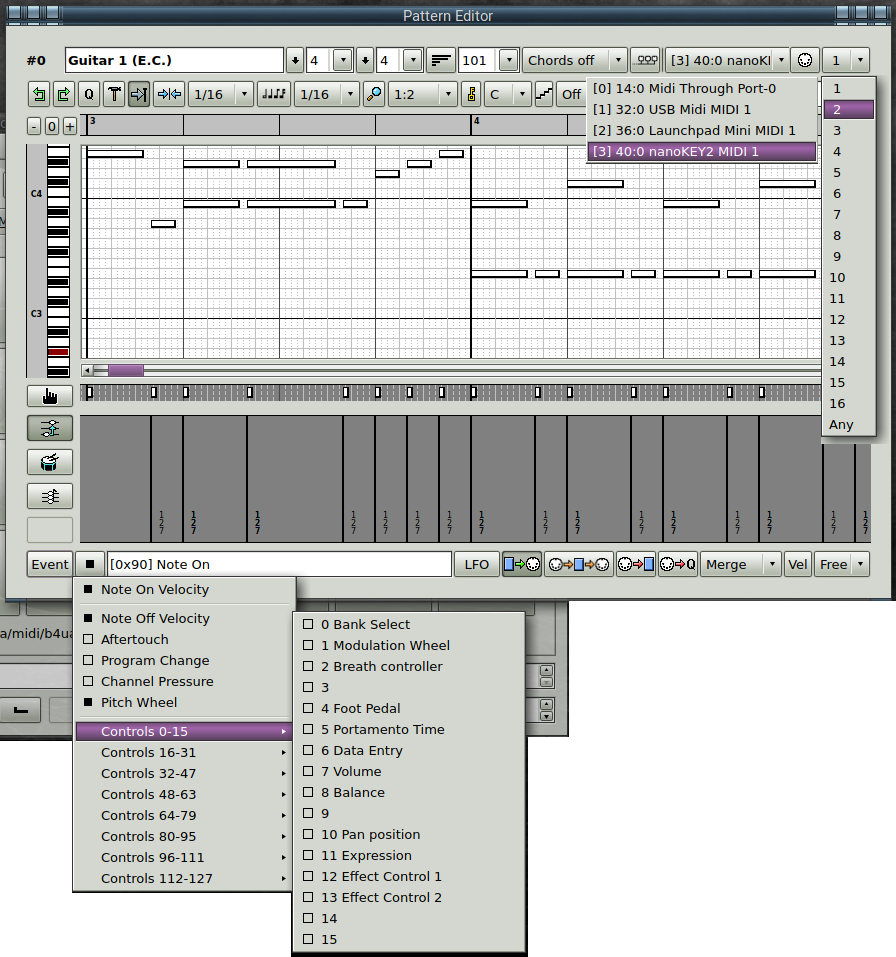
\includegraphics[scale=0.75]{configuration/usr/default-event-bus-channel-menus.png}
   \caption{Seq66 Composite View of Native Devices}
   \label{fig:default_event_bus_channel_menus}
\end{figure}

   At the top, the buss dropdown menu contains the MIDI busses/ports
   active on this computer.  At right, the MIDI channel shows
   the channels numbers that can be picked for buss 0.  At bottom left, we see
   the default controller values that \textsl{Seq66} includes.  We have
   no idea if these correspond to the controllers that the selected MIDI device
   supports.  We \textsl{can} use this dropdown to see if any such controller
   events are in the loaded MIDI file, of course; a solid black square
   indicates that such an event was found in the pattern.

   To change the default lists, we can create sections for busses and
   instruments in the 'usr' file.
   The discussion here relies on the reader opening the file
   \texttt{sample.usr}, which is included in the shared \texttt{data/samples}
   directory provided once \textsl{Seq66} is installed.

   Assume that we have 3 MIDI "buss" devices hooked to our system:
   two Model "2x2" MIDI port devices, and an old PCR-30 MIDI controller
   keyboard.  Let's number them, using the convention that buss numbers and
   channel numbers start at 0, not 1:

   \begin{itemize}
      \item 0. Model 2x2 A
      \item 1. Model 2x2 B
      \item 2. PCR-30
   \end{itemize}

   Then assume that we have nine different MIDI instruments in our kit.
   let's number them, too:

   \begin{itemize}
      \item 0. Waldorf Micro Q
      \item 1. SuperNova
      \item 2. DrumStation
      \item 3. TX81Z
      \item 4. WaveStation
      \item 5. ESI-2000
      \item 6. ES-1
      \item 7. ER-1
      \item 8. TB-303
   \end{itemize}

   The \textsl{Waldorf Micro Q},
   the \textsl{SuperNova},
   and the \textsl{DrumStation} all have a large
   number of special MIDI controller values for modifying the sound they
   produce.
   The \textsl{DrumStation} accepts MIDI controllers that change various
   features of the sound of each type of drum it supports.

   The buss devices shown here can be configured to route certain
   MIDI channels to certain MIDI devices.  Assume we have them
   set up this way:

   \begin{enumerate}
      \item Bus 0: Model 2x2 A
      \begin{itemize}
         \item SuperNova: channels 0 to 7
         \item TX81Z: channels 8 to 10
         \item Waldorf Micro Q: channels 11 to 14
         \item DrumStation: channel 15
      \end{itemize}
      \item Bus 1: Model 2x2 B
      \begin{itemize}
         \item WaveStation: channels 0 to 3
         \item ESI-2000: channels 4 to 13
         \item ES-1: channel 14
         \item ER-1: channel 15
      \end{itemize}
      \item Bus 2: PCR-30
      \begin{itemize}
         \item TB-303: channel 0
      \end{itemize}
   \end{enumerate}

   We use the \textbf{'usr' configuration file}.
   to show these items with the proper
   names associated with each device, channel, and controller value
   The process for setting up the 'usr' file is to:

   \begin{enumber}
      \item Define one or more MIDI busses, the name of each, and what
         instruments are on which channels.  Each buss is configured in a
         section of the form "\texttt{[user-midi-bus-X]}", where "X" ranges
         from 0 on up.  Each buss then defines up to 16 channel entries.
         Each entry includes the channel number and the number of a
         section in the user-instrument section described next.
      \item Define all of the instruments and their controller
         names, if they have them.  Each instrument is configured in a
         section of the form "\texttt{[user-instrument-X]}", where "X"
         ranges from 0 on up.  Up to 128 controllers can be defined.
   \end{enumber}

   Let's walk through the structure of this setup, since it is a little bit
   tricky.  Peruse the next couple of sections to understand a bit about the
   format of this file, following along in the sample 'usr' file.

\subsubsection{'usr' File / MIDI Bus Definitions}
\label{subsubsec:usr_file_midi_bus_definitions}

   \index{usr!user-midi-bus-definitions}
   \index{[user-midi-bus-definitions]}
   This section begins with an
   "INI" group marker \texttt{[user-midi-bus-definitions]}.
   It defines the number of user busses that will be configured in this file.
   This section contains an number
   of \texttt{[user-midi-bus-N]} sections, where "N" ranges from 0 on upward.
   These correspond to the MIDI \textsl{output}
   busses expected to be in the system (ignoring the ALSA "announce" buss if
   present).

   \begin{verbatim}
      [user-midi-bus-definitions]
      3     # number of user-defined MIDI busses
   \end{verbatim}

   \index{usr!user-midi-bus-n}
   \index{[user-midi-bus-n]}
   This means that the 'usr' file will have three MIDI buss
   sections:
   \texttt{[user-midi-bus-0]},
   \texttt{[user-midi-bus-1]}, and
   \texttt{[user-midi-bus-2]}.
   Here's is an example of one such buss section:

   \begin{verbatim}
      [user-midi-bus-0]
      2x2 A (SuperNova,Q,TX81Z,DrumStation)
      16
      0 1      # "channel" and "instrument number"
      1 1      # Instrument #1 of the [user-instrument-definitions] section
      . . .
      8 3      # Instrument #3 of the [user-instrument-definitions] section
      9 3
      . . .
      11 0     # Instrument #0 of the [user-instrument-definitions] section
      12 0     # This is the Waldorf Micro Q device
      . . .
      15 2     # Instrument #2 of the [user-instrument-definitions] section
   \end{verbatim}

   Each instrument is setup as a "channel" in a particular "buss".
   These instrument-definition sections are described in the next section.
   They are read from the 'usr' configuration file only if
   the "reveal ports" option is \textsl{off} ("0");
   this option can also be specified in the
   \texttt{[reveal-ports]} section of the 'rc' file.
   Otherwise, the actual port names reported by ALSA/JACK are shown.

   The \texttt{user-midi-bus-definitions} and \texttt{user-midi-bus-N} sections
   can be misleading if one wants to have access to the
   actual MIDI port names that exist on the system.
   It is left as an exercise for the reader to try these different combinations
   of show-port options.  Or one can consult the \textsl{Sequencer64 User
   Manual} to see the figures.

   \begin{itemize}
      \item Clocks View, -m (-{}-manual-ports)
      \item Inputs View, -m (-{}-manual-ports)
      \item Clocks View, -m (-{}-manual-ports) and -R (-{}-hide-ports)
      \item Clocks View, -r (-{}-reveal-ports)
      \item Inputs View, -r (-{}-reveal-ports)
      \item Clocks View, -R (-{}-hide-ports)
   \end{itemize}

\subsubsection{'usr' File / MIDI Instrument Definitions}
\label{subsubsec:usr_file_midi_instrument_definitions}

   \index{usr!user-instrument-definitions}
   \index{[user-instrument-definitions]}
   This section begins with an
   "INI" group marker \texttt{[user-instrument-definitions]}.
   It defines the number of user instruments that will be configured in this
   file.  This section defines characteristics, such as
   the meanings of MIDI controller values, of the instruments themselves,
   not the MIDI busses to which they attached.

   \begin{verbatim}
      [user-instrument-definitions]
      9     # number of user instruments
   \end{verbatim}

   \index{usr!user-instrument-n}
   \index{[user-instrument-n]}
   So this 'usr' file will define 9 instruments.  We provide only one section
   as an example.  Note that items without text default to the values
   prescribed by the General MIDI (GM) specification.

   Each instrument contains up
   to 128 controller values; these controller values are available in the
   \textbf{Event} button in the Pattern Editor, and their names are shown.

   \begin{verbatim}
      [user-instrument-0]
      Waldorf Micro Q                     # name of instrument
      128                                 # number of MIDI controllers
      0                                   # first controller value, unnamed
      1 Modulation Wheel
      2 Breath Control
      3 
      4 Foot Control
         . . .
      123 All Notes Off (0)
      124                                 # defaults to GM
      125 Unsupported
      126 Unsupported
      127                                 # defaults to GM
   \end{verbatim}

   Note the unnamed control numbers above.
   An unnamed control number might be an unsupported control number.
   It is termed to be "inactive".  In this case, the \textbf{Event} menu of
   the Pattern editor will show the default name of this controller.
   Again, though, the function denoted by this name might not be supported by
   the device.  In that case, it might be better to call it "Unsupported".
   See the examples above.  See the figure below for one example as set up using
   the \texttt{sample.usr} file:

\begin{figure}[H]
   \centering 
   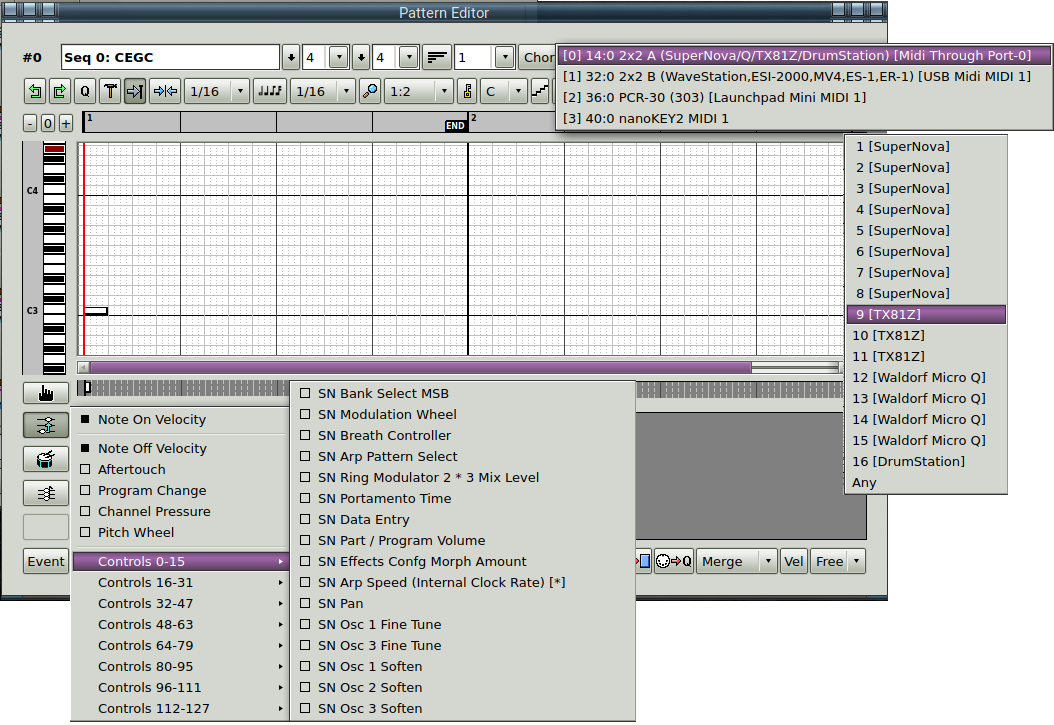
\includegraphics[scale=0.65]{configuration/usr/sample-usr-event-bus-channel-menus.png}
   \caption{Seq66 Composite View of Devices As Set in "sample.usr"}
   \label{fig:sample_usr_event_bus_channel_menus}
\end{figure}

\subsubsection{'usr' File / User Interface Settings}
\label{subsubsec:usr_file_user_interface_settings}

   \index{usr!user-interface-settings}
   \index{[user-interface-settings]}
   \index{usr!interface settings}
   This section, new to \textsl{Seq66}, begins with an
   "INI" group marker \texttt{[user-interface-settings]}.

   It provides for a feature we will hopefully be able to complete some day:
   the complete specificition of the appearance of the user-interface.
   There is plenty of room to change the appearance of
   \textsl{Seq66} already.
   Please try the settings and see what looks good.
   Refer to either the sample file or the file generated when \textsl{Seq66}
   first runs.

   \index{variset}
   \begin{verbatim}
      [user-interface-settings]
      swap-coordinates = false
      mainwnd-rows = 4
      mainwnd-columns = 8
      mainwnd-spacing = 2
      default-zoom = 2
      global-seq-feature = true
      progress-bar-thick = true
      inverse-colors = false
      window-redraw-rate = 40
      window-scale = 1
      window-scale-y = 1
   \end{verbatim}

   \texttt{swap-coordinates} allows for an alternate mapping of pattern
   numbers.  (Later, it will also apply to mappings for set-numbers and
   mute-group numbers.)  Here is the pattern layout:

   \begin{verbatim}
      [  0 ] [  1 ] [  2 ] [  3 ] [  4 ] [  5 ] [  6 ] [  7 ]
      [  8 ] [  9 ] [ 10 ] [ 11 ] [ 12 ] [ 13 ] [ 14 ] [ 15 ]
      [ 16 ] [ 17 ] [ 18 ] [ 19 ] [ 20 ] [ 21 ] [ 22 ] [ 23 ]
      [ 24 ] [ 25 ] [ 26 ] [ 27 ] [ 28 ] [ 29 ] [ 30 ] [ 31 ]
   \end{verbatim}

   Compare it to the layout shown in
   \sectionref{paragraph:patterns_pattern_keys}.
   Note that \texttt{progress-bar-thick} also applies to the box that hold the
   notes and progress-bar in the Live grid buttons.
   There are a number of additional user-interface options.  See the generated
   or sample 'usr' file for descriptions.  Also see the chapter on palettes.

\subsubsection{'usr' File / User MIDI PPQN}
\label{subsubsec:usr_file_user_midi_ppqn}

   The long-standing PPQN for \textsl{Seq24} was a value of 192, and
   \textsl{Seq66} sticks with that default.
   This value is good for most tunes. But other sequencers allow for higher
   values. \textsl{Seq66} allows for some crazy values, ranging from
   32 to 19200.  If a MIDI file has a different PPQN, it will be rescaled to
   the default PPQN.  However, one might want to stick with the PPQN
   specified in the MIDI file, so \textsl{Seq66} allows that as well.
   It is probably best to set \texttt{use-file-ppqn = true}, but that is
   up to the user.

   \index{usr!midi-ppqn}
   \index{default PPQN}
   \index{file PPQN}
   \begin{verbatim}
      [user-midi-ppqn]
      default-ppqn = 192
      use-file-ppqn = true
   \end{verbatim}

\subsubsection{'usr' File / User MIDI Settings}
\label{subsubsec:usr_file_user_midi_settings}

   \index{[user-midi-settings]}
   This section begins with an
   "INI" group marker \texttt{[user-midi-settings]}.
   It allows one to specify the
   global defaults for tempo, beats per measure, and so on.

   \index{usr!convert-to-smf-1}
   \index{usr!beats-per-bar}
   \index{usr!beats-per-minute}
   \index{usr!beat-width}
   \index{usr!buss-override}
   \index{usr!velocity-override}
   \index{usr!bpm-precision}
   \index{usr!bpm-step-increment}
   \index{usr!bpm-page-increment}
   \index{usr!bpm-minimum}
   \index{usr!bpm-maximum}
   \begin{verbatim}
      [user-midi-settings]
      convert-to-smf-1 = true
      beats-per-bar = 4
      beats-per-minute = 120
      beat-width = 4
      buss-override = -1
      velocity-override = 80     # velocity_override (-1 = 'Free')
      bpm-precision = 1          # 0, 1, or 2
      bpm-step-increment = 0.1
      bpm-page-increment = 5.0
      bpm-minimum = 0
      bpm-maximum = 127
   \end{verbatim}

   The \texttt{convert-to-smf-1} option is normally true. This causes
   \textsl{Seq66} to convert single track MIDI files (in SMF 0 format) to
   multi-track SMF 1 files.

   \index{port!override}
   \index{buss!override}
   The \texttt{buss-override} option causes the buss-value (port number) to be
   applied to each pattern in a MIDI song that is loaded.  This allows the tune
   to be directed to one's favorite synthesizer/application.
   Unlike the global port override in the main window
   (see \sectionref{subsubsec:introduction_sets_buss_override}),
   this application does not modify the file, though one can still opt to save
   it, which locks in the new buss number.

   The \texttt{velocity-override} option fixes a long standing (from
   \textsl{Seq24}) bug where the actual incoming note velocity was always
   replaced by a hard-wired value.  A value of "-1" corresponds to the "Free"
   setting, which preserves the incoming velocity.

   The \texttt{bpm-precision}, \texttt{bpm-step-increment}, and
   \texttt{bpm-page-increment} values allow more precise control over tempo,
   which makes it easier to match the tempo of external music sources.  Note
   that the step-increment is used by the up/down arrow buttons, the up/down
   arrow keys, and the MIDI BPM control values.  The page-increment is used
   if the BPM field has focus and the Page-Up/Page-Down keys are pressed,
   and new MIDI control values have been added to support coarse MIDI
   control of tempo.

   The \texttt{bpm-minimum} and \texttt{bpm-maximum} settings
   are used in scaling the display of Tempo events.
   By adjusting these values, one can more easily see the variations in
   tempo.  In a main window pattern slot, or in the song editor tempo track,
   this range is scaled to the full range of note values, 0 to 127.
   Generally, one wants to select a range that keeps the main tempo line at
   the middle height of the pattern display.

   To obtain these new settings, remember to backup the existing
   \textsl{seq66.usr}, then run \textsl{Seq66} with the
   \texttt{-{}-user-save} option, and then do a "diff" on the new file and the
   original to merge any old values that need to be preserved.  Then make any
   further tweaks to the new values.

\subsubsection{'usr' File / User Options}
\label{subsubsec:usr_file_user_options}

   \index{[user-options]}
   This section begins with an
   "INI" group marker \texttt{[user-options]}.
   It provides for additional options keyed by the
   \texttt{-o}/\texttt{-{}-option} options.
   This group of options serves to expand the options that are available, since
   \textsl{Seq66} is running out of single-character options.
   This group of options are shown below.

   \index{usr!option-daemonize}
   \index{usr!option-logfile}
   \index{usr!option-pdf-viewer}
   \index{usr!option-browser}
   \begin{verbatim}
      [user-options]
      daemonize = false
      log = "seq66.log"
      pdf-viewer = "/usr/bin/zathura"
      browser = "/usr/bin/lynx"
   \end{verbatim}

   If this option is not used when running \texttt{seq66cli}, then the
   application stays in the console window and dumps informational output to
   it.  If this option is in force, then the only way to affect
   \texttt{seq66cli} is to send a signal (e.g. SIGKILL) to it, or use
   MIDI control.
   However, currently we have issue with this option, so one should run
   \texttt{seq66cli} in the background from a console or from a desktop shortcut.

   The log-file, if specified, is written to the same directory as the 'usr'
   file, the \textsl{Seq66} configuration directory.
   If empty, then a valid file-name can be specified
   in the \texttt{-{}-option log=filename.log} option.
%  There's more to the 'usr' configuration file than we've exposed here.

   The PDF viewer and browser options are used if non-empty.
   Otherwise, the system default applications are used.

\subsubsection{'usr' File / Additional Options}
\label{subsubsec:usr_file_added_options}

   \textbf{\texttt{[user-work-arounds]}} is a section that is a relic from
   older versions of this application.  It can be ignored.  More useful options
   are described below.

\paragraph{'usr' File / Additional Options / [user-ui-tweaks]}
\label{paragraph:user_file_added_options_tweaks}

   \texttt{[user-ui-tweaks]} provides a small number of tweaks to the
   user-interface.

   \begin{verbatim}
      [user-ui-tweaks]
      key-height = 10
      note-resume = false
      style-sheet = "qseq66.qss"    # optional, can include a path
      fingerprint-size = 128
      progress-box-width = 0.8
      progress-box-height = 0.4
      progress-box-shown = true
      progress-note-min = 20
      progress-note-max = 100
      lock-main-window = true
   \end{verbatim}

   \index{key height}
   The \texttt{key-height} option
   affects the default "width" of the piano keys in the pattern
   sequence editor.  Defaults to 12 (pixels).
   This option is also editable in the \textbf{Preferences} dialog.
   There are vertical zoom buttons, and the \texttt{v/0/V} keystrokes to change
   this on the fly, but those changes are not saved.

   \index{new seqedit}
   \textsl{Seq66} now uses the new pattern editor in the 'Edit' tab.
   When used in the \textbf{Edit} tab instead of an external window,
   it is shrunk slight vertically, but the bottom row of buttons is invisible
   unless the user makes the window taller.
   The old smaller pattern editor is less functional and a bit more buggy.
   It has gone away completely.

   The following options adopt the new convention for setting variables, in
   which the format is \texttt{item-name = value}.
   This style will eventually be used for all settings.

   \index{note resume}
   The \texttt{note-resume} option, if active, causes any notes in progress
   to be resumed when the pattern is toggled back on.

   \index{style sheet}
   The \texttt{style-sheet} option, if non-empty, causes a user-designed
   style-sheet to be applied.  This is useful in expanding the tab-sizes,
   or making disabled text easier to read in some Qt themes.
   See \texttt{data/samples/textfix.qss} for an example.
   The style sheet file is assumed to reside in the normal \textsl{Seq66}
   configuration directory.
   However, it can have a path component so that the same style sheet
   can be used by many applications more readily.
   Here is an example using the style sheet file
   \texttt{data/samples/qseq66.qss}:

\begin{figure}[H]
   \centering 
   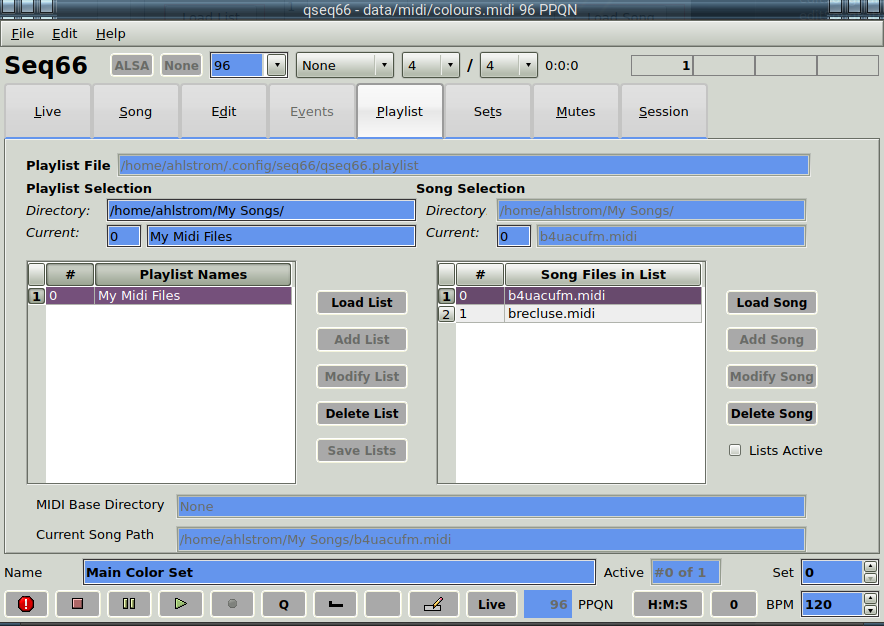
\includegraphics[scale=0.75]{main-window/main-window-stylesheet.png}
   \caption{Seq66 View with Style Sheet Applied}
   \label{fig:view_with_style_sheet_applied}
\end{figure}

   Note the blue text fields. Also note the larger tabs, which could be useful
   on a touch-screen.
   There is a full-scale dark theme stored in
   \texttt{data/win/dark-theme.qss}.
   One might want to save and tweak the 'palette' file to match.

   \index{fingerprint}
   The \texttt{fingerprint} option provides a way to reduce the amount of
   drawing in the pattern grid.  The pattern box in each button is small, and,
   for patterns longer than the fingerprint size, it makes no sense to draw
   hundreds of notes.  Instead, patterns shorter than the fingerprint size are
   drawn normally, while longer patterns are drawn with a "fingerprint", a
   compressed representation of the pattern.

   \index{progress box!width}
   \index{progress box!height}
   The \texttt{progress-box-width} and
   The \texttt{progress-box-height} options provide a way to expand or reduce
   the size of the progess box in each grid button.
   It is purely a user preference.
   The width ranges from 0.5 to 1.0 (full size), with a default of 0.8.
   The height ranges from 0.1 to 1.0 (full size), with a default 0f 0.3.
   Try setting both the width and height to 0.9 for an interesting effect.

%  If either is 0, then the box isn't drawn, and the pattern appears directly
%  on the button.

   \index{progress box!shown}
   If  \texttt{progress-box-shown} is false, then the progress boxes are not
   drawn, and the pattern appears directly on the button.

   \index{progress-note-min}
   \index{progress!note-min}
   \index{progress-note-max}
   \index{progress!note-max}
   The \texttt{progress-note-min} and
   The \texttt{progress-note-max} options change the note range in the progress
   box to control where in "pitch" the notes are shown.

   \index{lock-main-window}
   The \texttt{lock-main-window} option, if true, prevents the main window from
   being resized.  It can still be moved, and the external pattern and song
   editors can still be resized.

\paragraph{'usr' File / Additional Options / [user-session]}
\label{paragraph:user_file_added_options_session}

   \texttt{[user-session]} provides a way to cooperate with the
   \textsl{Non Session Manager}.
   See \sectionref{subsec:sessions_nsm_before_using_nsm}; it goes into great
   detail.

   \begin{verbatim}
      [user-session]
      session = none
      url = ""
   \end{verbatim}

\paragraph{'usr' File / Additional Options / [new-pattern-editor]}
\label{paragraph:user_file_added_options_pattern_editor}

   \texttt{[new-pattern-editor]} contains settings values for recording
    when a new pattern editor is opened. A new pattern is indicated when
   the loop has the default name, \textsl{Unititled}.
    These values save time during a live recording session.
   The valid values for record-style are \texttt{merge},
    \texttt{overwrite}, and \texttt{expand}.

   \begin{verbatim}
      [new-pattern-editor]
      armed = false
      thru = false
      record = false
      qrecord = false
      record-style = merge
      wrap-around = false
   \end{verbatim}

   Also included is a flag to allow notes to wrap around, where the Note On
   comes near the end of the pattern, but the Note Off appears after the
   pattern loops back to the beginning.
   If false, then two unlinked note events appear in the piano roll, colored
   magenta.  The "u" command in the piano roll will remove them.
   If one does not want to deal with wrap-around at all, then set the pattern
   length to the desired measure count \textsl{plus one} while recording, until
   satisfied with the recording.  Shrink or delete any notes that bleed into
   the extra measure. Then set the pattern back to the desired length.

\subsection{'ctrl' File}
\label{subsec:configuration_ctrl}

   \textsl{Seq66} provides a way to control the
   application to some extent via a MIDI controller, such as a MIDI keyboard or
   a MIDI pad.  The current section describes this feature;
   additional resources and ideas can be found at \url{linuxaudio.org}
   \cite{midicontrol}.
   Also see the tutorial section \sectionref{sec:launchpad_mini}.
   An \textsl{Open Document Format} spreadsheet in the
   \texttt{doc} directory shows layouts for the default
   keystroke configuration (including pattern, mutes, and automation controls)
   and for a couple of \textsl{Launchpad Mini} configurations.
   Another spreadsheet lists the support names for keys; these names can be used
   in the 'ctrl' file, and include some changes for French AZERTY keyboards.
   The spreadsheets are
   \texttt{control\_keys.ods} and
   \texttt{launchpad-mini.ods}.

   The 'ctrl' file provides settings for keyboard control, MIDI control, and
   for specifying MIDI output to reflect \textsl{automation} commands in a
   device such as the \textsl{LaunchPad Mini}.  The name of this file and its
   active status are specfied in the 'rc' file as noted earlier.

\subsubsection{'ctrl' File / MIDI Control Settings}
\label{subsubsec:configuration_ctrl_midi_control_settings}

   \begin{verbatim}
      /home/user/.config/seq66/qseq66.usr             (Linux)
      C:/Users/user/AppData/Local/seq66/qpseq66.usr   (Windows)
   \end{verbatim}

   This file offloads the control settings from the 'rc' file, for a more
   flexible setup. It starts with the sections common to all \textsl{Seq66}
   configuration files.  The first unique section defines some useful settings
   using the new variables feature of the configuration.  Look at the sample or
   generated file to see the layout of these items.

   \begin{verbatim}
      [midi-control-settings]
      control-buss = 3              # or 0xff
      midi-enabled = true
      button-offset = 0
      button-rows = 4
      button-columns = 8
      keyboard-layout = qwerty
   \end{verbatim}

   \begin{itemize}
      \item \texttt{control-buss}.
         The control-buss value ranges from 0 to the maximum buss provided by
         the hardware on the system. If set, then only that buss will be allowed
         to send MIDI control.  A value of 255 or 0xff means any buss can send
         MIDI control. If port-mapping is enabled, the short name (nick-name) of
         the port can be used.
      \item \texttt{midi-enabled}.
         If set to "true", then the MIDI controls will be used.
         It can be set to "false", while keeping the configuration in place
         for later usage.
      \item \texttt{button-offset}.
         This item provides a way to move a set of input controls (e.g. from a
         \textsl{Launchpad Mini}) to a different area of the input control
         device.  Not yet supported.
      \item \texttt{button-rows}.
         Indicates the rows of the input control grid.
         Still in progress.
      \item \texttt{button-columns}.
         Indicates the columns of the input control grid.
         Still in progress.
      \item \texttt{keyboard-layout}.
         Provides a way to adapt to non-US keyboards.
         Currently, the only supported values are "normal" ("qwerty"), "qwertzy",
         and "azerty".
         For "azerty", the auto-shift feature of group-learning is disabled.
         The handling of keyboards can be quite complex, and differ between
         Linux distros and Windows.
         Especially problematic are the "dead keys" supported by some locales.
   \end{itemize}

\subsubsection{'ctrl' File / Loop Control}
\label{subsubsec:configuration_ctrl_loop_control}

   The loop-control group consists of 32 lines (0 to 31), one for each
   pattern slot shown in the patterns panel.
   It provides a way to control the arming/disarming (muting/unmuting) of
   each pattern shown in the patterns panel.
   It consolidates the keyboard and MIDI control settings into one table.

   Note that the main window shows the \textsl{active} screen-set.
   These MIDI controls affect the \textsl{active} screen-set.

   This block of matrix elements, numbered from 0 to 31,
   represent control functions (toggle, mute, unmute) for the 32 patterns
   of the active screen-set.
   These 32 rows correspond to the hot-keys assigned in
   the \textbf{File / Options / Keyboard / Control keys [keyboard-group]} 
   configuration panel.

   \index{[loop-control]}
   The MIDI control section begins with the following "INI"-style
   group marker tag, followed by one stanza-line per loop:

   \begin{verbatim}
      [loop-control]
      # Control:  Toggle          On               Off
       0 "1"     [ 0 0x00 0 0 0 ] [ 0 0x00 0 0 0 ] [ 0 0x00 0 0 0 ] # Loop 0
       1 "q"     [ 0 0x00 0 0 0 ] [ 0 0x00 0 0 0 ] [ 0 0x00 0 0 0 ] # Loop 1
       . . .
      31 ","     [ 0 0x00 0 0 0 ] [ 0 0x00 0 0 0 ] [ 0 0x00 0 0 0 ] # Loop 31
   \end{verbatim}

   The first column is an index number, starting at 0.  It indicates what
   loop the control line will affect.
   \index{keys!control}
   The second column is the name of the keystroke that will act as a toggle or
   action key.
   \index{keys!blank}
   If the key name is \texttt{Blank}, then there is no keystroke for that
   pattern control.  The user can specify multiple blank keys as desired.

   The numbers in the leftmost brackets define a \textsl{Toggle} control;
   the numbers in the middle brackets define an \textsl{On} control;
   the numbers in the rightmost brackets define an \textsl{Off} control.
   The numbers inside each set of brackets define six values that set up the
   control.  The layout of each filter inside the brackets is as follows:

      \textbf{[INV STAT D1 D2min D2max]}

   \begin{itemize}
      \item \textbf{INV} = \textbf{inverse}
      \item \textbf{STAT} = \textbf{MIDI status byte} (channel included) 
      \item \textbf{D1} = \textbf{data1}
      \item \textbf{D2min} = \textbf{data2 min}
      \item \textbf{D2max} = \textbf{data2 max}
   \end{itemize}

   If \textbf{STAT} is not 0x00, the control is enabled.  \textsl{Seq66} will
   match the incoming MIDI event against the \textbf{STAT (MIDI status byte)}
   pattern (e.g. a Note On event), and perform the action (On/Off/Toggle) if
   the \textbf{D1} (e.g. a Note number), matches the incoming data, and the
   incoming parameters (e.g. Note velocity) falls in the specified
   \textbf{D2min} to \textbf{D2max} range.  All data values are best specified
   in decimal.

   The \textbf{INV (inverse)} field will make the pattern perform the opposite
   action (\textsl{off} for \textsl{on}, \textsl{on} for \textsl{off}) if the
   data falls outside the specified range.  This is cool because one can map
   several sequences to a knob or fader.

   The \textbf{STAT (MIDI status byte)} field is a MIDI status byte number in
   decimal or hexadecimal notation.
   Remember that it can include a channel.  This channel is not overridden by
   the pattern's selected channel when a MIDI control matching event is
   received. 
%  The channel nybble of this byte is ignored.
   One can look up the possible status values up in the MIDI messages tables;
   the relevant data can be found at \cite{midicontroltable}.
%  As the channel on which the events are sent is ignored,
%  it is sufficient to use the values for channel 1; that is, 0.

   The last three fields describe the range of data that will match.  The
   \textbf{D1 (data1)} field provides the actual MIDI event message number to
   detect, in decimal.  This item could be a Note On/Off event or a
   Control/Mode change event, for example.
   The \textbf{D2min (data2 min)} field is the minimum value of the event for
   the filter to match. For Note On/Off events, this would be the velocity
   value, for example.
   The \textbf{D2max (data2 max)} field is the maximum value of the event for
   the filter to match.

%  This set of values is explained below.

   For each pattern, we can set up MIDI events to turn a 
   pattern on, off, or to toggle it.
   The loop MIDI control setup resembles a matrix.  The default matrix
   uses the central keys on the keyboard, laid out in a 4 x 8 grid matching the
   pattern buttons:

   \begin{verbatim}
      1 2 3 4 5 6 7 8
      q w e r t y u i
      a s d f g h j k
      z x c v b n m <
   \end{verbatim}

   Please note that the buttons on some (or most) MIDI controllers send a
   message on press and another message on release.  One can set such buttons
   up as toggle buttons by defining only the "Toggle" (first) stanza.
   Or one can have the button active the function on press, and then deactivate
   it on release by defining the "On" (second) and "Off" (third) stanzas
   appropriately.

\subsubsection{'ctrl' File / Mute-Group Control}
\label{subsubsec:configuration_ctrl_mute_group_control}

   \index{mute-group control}
   This section provides controls for 32 groups of mutes.
   A group is a set of patterns that can toggle their playing state
   together.  Every group contains all 32 sequences in the active screen set.
   So, this part of the MIDI Control section is used for muting and unmuting
   (and toggling) a group of patterns using a keystroke or MIDI control.
   The definitions are in the same format as the loop-control section.

   \begin{verbatim}
      [mute-group-control]
        0 "!"  [ 0 0x00 0 0 0 ] [ 0 0x00 0 0 0 ] [ 0 0x00 0 0 0 ] # Mute 0
        1 "Q"  [ 0 0x00 0 0 0 ] [ 0 0x00 0 0 0 ] [ 0 0x00 0 0 0 ] # Mute 1
       . . .
       31 "<" [ 0 0x00 0 0 0 ] [ 0 0x00 0 0 0 ] [ 0 0x00 0 0 0 ]  # Mute 31
   \end{verbatim}

   All this section does is set up the controls to be used; the actual
   mute-group patterns are defined in the 'mutes' configuration file (or in the
   \textsl{Seq66} MIDI file itself.
   A key name of \texttt{Blank} can be used to disable a keystroke for
   that line.

   The mutes MIDI control setup resembles a matrix match the shifted versions
   of the loop control keys.  The default matrix
   uses the central keys on the keyboard, laid out in a 4 x 8 grid matching the
   pattern buttons:

   \begin{verbatim}
      ! @ # $ % ^ & *
      Q W E R T Y U I
      A S D F G H J K
      Z X C V B N M <
   \end{verbatim}

\subsubsection{'ctrl' File / Automation Control}
\label{subsubsec:configuration_midi_ctrl_automation}

   This section provides ways to control \textsl{Seq66} push-button controls
   from a keyboard or from a MIDI device.
   These entries control
   \textsl{Seq66} actions like changing the BPM value, screen-set,
   record, solo, etc.

   Note that automation controls that depend upon a parameter (such as group
   number or loop number) can only work with a MIDI control.
   MIDI control can provide parameters via a control value, note number or value,
   etc.
   Key control can provide only a "press" or "release" status.
   
   Each item in this group consists of one line.  Each line
   specifies a MIDI event that can cause a given
   \textsl{Seq66} user-interface operation to occur.
   These items are easy to view in the 'ctrl' configuration file,
   in the \texttt{[automation-control]} section.

   \begin{verbatim}
      [automation-control]
       0 "'"    [ 0 0x00 0 0 0 ] [ 0 0x00 0 0 0 ] [ 0 0x00 0 0 0 ]  # BPM Up
       1 ";"    [ 0 0x00 0 0 0 ] [ 0 0x00 0 0 0 ] [ 0 0x00 0 0 0 ]  # BPM Dn
       . . .
      35 "Quit" [ 0 0x00 0 0 0 ] [ 0 0x00 0 0 0 ] [ 0 0x00 0 0 0 ]  # Loop 0
       . . .
      48 "0xfe" [ 0 0x00 0 0 0 ] [ 0 0x00 0 0 0 ] [ 0 0x00 0 0 0 ]   # Reserved 48
   \end{verbatim}

   Note that "Quit" is not a real keystroke.  It is a placeholder in the internal
   keystroke map for the functionality of quitting \textsl{Seq66} via MIDI
   control.  Qt provides other ways to quit via keystroke.
   A key name of \texttt{Blank} can be used to disable a keystroke for
   a line.
   The stanzas meaning can change depending on the type of control.  Here are
   the important styles:

   \begin{verbatim}
      Normal:        [ Toggle       ] [ On          ] [ Off             ]
      Playback:      [ Pause Play   ] [ Start Play  ] [ Stop Play       ]
      Play list:     [ Select by D2 ] [ Select Next ] [ Select Previous ]
      Play song:     [ Select by D2 ] [ Select Next ] [ Select Previous ]
   \end{verbatim}

   For selecting play-lists and songs by number, \textbf{D2} is used.
   Thus, one possible value to use to select would be to use a 
   Note On event on channel 16 (0x9F) with a note number of 0 (a rarely-used
   note in any tune), and list/song numbers ranging from 0 to 127.  Using note
   0 for list selection and note 1 for song selection:

   \begin{verbatim}
      24 "F2" [ 0 0x9F   0   0 127 ] [ . . . ] [ . . .] # Play List
      25 "F3" [ 0 0x9F   1   0 127 ] [ . . . ] [ . . .] # Play Song
   \end{verbatim}

   Obviously, this requires a MIDI controller for which the velocity can be
   exactly specified.  One can also reserve \textbf{D2} values of 126 for
   "previous" and 127 for "next".

\paragraph{Automation / BPM Up and Down}
\label{paragraph:configuration_midi_ctrl_bpmupdn}

   These controls increment or decrement the beats-per-minute setting, as if
   the up- or down-arrow has been clicked in the BPM combox-box, or the up- or
   down-arrow key pressed, in that combo-box.
   This increment is the
   \index{bpm!step increment}
   \index{usr!step increment}
   "step increment" which defaults to 1, but can be modified by
   changing the "bpm\_step\_increment" value in the 'usr'
   configuration file.

\paragraph{Automation / Screen-Set Up and Down}
\label{paragraph:configuration_midi_ctrl_ssupdn}

   Also abbreviated "Set Up" and "Set Down".
   This control increments / decrements to the next / previous screen-set. 
   Once the screen-set has been altered, mute-groups and other
   actions apply to that screen set.

\paragraph{Automation / Mod Replace}
\label{paragraph:configuration_midi_ctrl_modrep}

   This control the "replace" flag.
   Then, when the user manually clicks a pattern slot,
   that pattern is unmuted, and all the rest are muted.
   Thus, this MIDI control is kind a of "Solo" function.
   It works whether in "Live" or "Song" mode.

\paragraph{Automation / Mod Snaphot}
\label{paragraph:configuration_midi_ctrl_modsnap}

   This control causes the playing statuses of all active
   (i.e. having data) patterns to be saved.  When turned off, the
   original playing status is restored.  Thus, two MIDI events
   need to be allocated to this functionality.

\paragraph{Automation / Mod Queue}
\label{paragraph:configuration_midi_ctrl_modqueue}

   This control sets up the "queue" status flag.
   Then, when the user manually clicks a pattern slot,
   that pattern is queued, and will play at the next cycle of the
   pattern.

   Here is an example from \cite{midicontrol}, which shows how to set up
   the "Sustain" control-change event to queue or un-queue a sequence:
   The \textsl{Akai MPK Mini} has a Sustain button and we can set the
   Sustain MIDI event (with MIDI status byte 176 [0xB0] to represent a
   Controller event, and control/mode change number 64 [0x40] to
   represent the Sustain or Pedal control) up as the queue modifier in
   the \texttt{mod queue} entry:

   \begin{verbatim}
      6 "o" [ 0  0x00 0  0  0 ] [ 0  0xB0 64 127 127 ] [ 0  0xB0 64 0  0 ]
      #      INV STA  D1 mn mx   INV STA  D1 mn  mx     INV STA D1  mn mx
      #                                   ^  ^                      ^  ^
      #                                   |  |                      |  |
      #                                   |   ----Sustain-----------   |
      #                                    -------Control Change-------
   \end{verbatim}

   So when the Sustain button is held down, and one presses one of the pads
   on the \textsl{MPK Mini}, the corresponding sequence gets queued.
   Also included in the data directory are sample 'ctrl' files for other devices.

\paragraph{Automation / Mute Group}
\label{paragraph:configuration_midi_ctrl_modgmute}

   This MIDI control sets up a "group learn".
   This control sets two internal flags on : "mode-group" and "group-learn".
   The first flag indicates that we will be handling mute-groups.
   The second flag indicates that we are learning these mute-groups,
   effectively recording the current status of all the patterns in all of the
   screen-sets.

   \index{L button}
   Note that this control corresponds to the "L" button in the main window
   user-interface.
   \index{keys!l}
   It can also be accessed by the default hot-key, \texttt{l}.
   Note that, once in learn-mode, there is no way to cancel learn-mode
   except by selecting an illegal mute-group keystroke.
   Also see \sectionref{sec:mutes_master}.

\paragraph{Automation / Record Modes and Quantization}
\label{paragraph:configuration_midi_record_quan}

   For release 0.97.3,
   \index{patterns-panel!modes}
   \index{grid modes}
   \textbf{grid modes} have been introduced.
   The \textbf{Record} and \textbf{Quan Record} automation controls have been
   refactored to cycle through these modes.
   Additional automation commands provide direct access to each mode.

   Grid mode changes the function of the main window's patterns panel so that
   it can be used to initiate record instead of toggling mute status,
   regardless of whether the toggling is done via the buttons, hot-keys, or
   MIDI controls.  The following modes are supported:

   \begin{itemize}
      \item \textbf{Loop}.
      \item \textbf{Record}.
      \item \textbf{Copy}.
      \item \textbf{Paste}.
      \item \textbf{Clear}.
      \item \textbf{Delete}.
      \item \textbf{Thru}.
      \item \textbf{Solo}.
      \item \textbf{Cut}.
      \item \textbf{Double}.
   \end{itemize}

   A click or a hot-key will cause the selected function above to be applied to
   the pattern denoted by the click/key.
   For details, see \sectionref{paragraph:patterns_recording_modes}.
   In \textbf{Record} mode, the following settings are enabled:

   \begin{itemize}
      \item \textbf{Overdub}.
      \item \textbf{Overwrite}.
      \item \textbf{Expand}.
      \item \textbf{One-shot}.
      \item \textbf{One-shot Reset}.
   \end{itemize}

   For details, see \sectionref{paragraph:patterns_recording_modes}.
   Also supported is changing the mode of recording:

   \begin{itemize}
      \item \textbf{No Quan}.
      \item \textbf{Quantize}.
      \item \textbf{Tighten}.
      \end{itemize}

   For details, see \sectionref{paragraph:patterns_recording_modes}.
   Also see \sectionref{subsec:pattern_editor_bottom} for more information on these
   recording modes.

\paragraph{Automation / Screen-Set Play}
\label{paragraph:configuration_midi_ctrl_ssplay}

This MIDI control sets the playing screen-set.

\subsubsection{Automation / More MIDI Control}
\label{subsubsec:configuration_midi_ctrl_automationex}

   Many additional control items were requested by users, to control
   additional features of the application.  Too many to list here.
   See the 'ctrl' file samples for more information.

\subsubsection{'ctrl' File / MIDI Control Output}
\label{subsubsec:configuration_ctrl_midi_control_out}

   This section provides a way to have a MIDI device, such as the
   \textsl{Novation Launchpad Mini}, show the status
   of the patterns that are active, as well as other information.
   The first sub-section sets up some general settings.

   \begin{verbatim}
      [midi-control-out-settings]
      set-size = 32
      output-buss = 1
      midi-enabled = true
      button-offset = 0
      button-rows = 8
      button-columns = 8
   \end{verbatim}

   \begin{itemize}
      \item \texttt{set-size}.
         Provides the set size.  The default is 32, in a 4 x 8 grid.
      \item \texttt{output-buss}.
         Indicates where automation-display controls are to be sent.
         Specify the output buss to which the display device is attached. If
         port-mapping is enabled, the short name (nick-name) of the port can be
         used.
      \item \texttt{midi-enabled}.
         If set to "true", then the MIDI control outputs will be used.
         It can be set to "false", while keeping the configuration in place
         for later usage.
      \item \texttt{button-offset}.
         This item provides a way to move a set of output controls (e.g. from a
         \textsl{Launchpad Mini}) to a different area of the output control
         device.  Not yet supported.
      \item \texttt{button-rows}.
         Indicates the rows of the output control grid.
         Still in progress.
      \item \texttt{button-columns}.
         Indicates the columns of the output control grid.
         Still in progress.
   \end{itemize}

   \begin{verbatim}
      [midi-control-out]
       0 [ 0x90  0 60 ] [ 0x90  0 15 ] [ 0x90  0 62 ] [ 0 0x90  0 12 ]
       1 [ 0x90  1 60 ] [ 0x90  1 15 ] [ 0x90  1 62 ] [ 0 0x90  1 12 ]
      . . .
      31 [ 0x90 31 60 ] [ 0x90 31 15 ] [ 0x90 31 62 ] [ 0 0x90 31 12 ]
   \end{verbatim}

   The first number is the pattern number of the pattern whose armed/muted
   status is to be shown.
   There are samples in the \texttt{data/linux} directory for some devices that
   one can adapt to other equipment.
   The mute-group buttons and their status can also be shown:

   \begin{verbatim}
      [mute-control-out]
       0 [ 0x00   0   0 ] [ 0x00   0   0 ] [ 0x00   0   0 ]
       1 [ 0x00   0   0 ] [ 0x00   0   0 ] [ 0x00   0   0 ]
        . . .
      31 [ 0x00   0   0 ] [ 0x00   0   0 ] [ 0x00   0   0 ]
   \end{verbatim}

   There are additional automation controls whose status can be displayed:

   \begin{verbatim}
      [automation-control-out]
      0 [ 0x00   0   0 ] [ 0x00   0   0 ] [ 0x00   0   0 ]  # Panic
      0 [ 0x00   0   0 ] [ 0x00   0   0 ] [ 0x00   0   0 ]  # Stop
       . . .
      0 [ 0x00   0   0 ] [ 0x00   0   0 ] [ 0x00   0   0 ]  # Tap_BPM
      0 [ 0x00   0   0 ] [ 0x00   0   0 ] [ 0x00   0   0 ]  # Quit
   \end{verbatim}

   See the sample files for more detailed descriptions.
   Also see \sectionref{sec:launchpad_mini}; it showns a fairly comprehensive
   setup based on the file \texttt{data/linux/qseq66-lp-mini.ctrl}.

\subsubsection{'ctrl' File / Macro Control Output}
\label{subsubsec:configuration_ctrl_macro_control_out}

   This section provides a way to send setup information to a MIDI device,
   such as the \textsl{Novation Launchpad Pro Mk3}.
   There is too much involved (especially that device) to discuss in
   detail here, but this feature can be used to put a device into
   "programmer" mode at \textsl{Seq66} startup and back into
   "normal" mode at \textsl{Seq66} shutdown.
   Here is a hypothetical sample for the Mk3:

   \begin{verbatim}
      [macro-control-out]
      footer = 0xf7
      header =0xf0 0x00 0x20 0x29 0x02 0x0e 
      reset = $shutdown
      shutdown = $live-mode
      startup = $programmer-mode
      live-mode = $header 0x0e 0x00 $footer
      programmer-mode = $header 0x0e 0x01 $footer
   \end{verbatim}

   The macros "footer", "header", "reset", "startup", and "shutdown"
   are written to the 'ctrl' file if not already present, though
   they won't have any useful definition.
   The first three are useful in other macros, while "startup" and
   "shutdown", if defined with actual data, are sent at the launch
   and shutdown, respectively, of \textsl{Seq66}.
   Note that these macros can be re-used in other macros, to
   increase the readability of the macros and to reduce the
   chance for mistakes.
   Note, too, that many devices required a device-specific
   SysEx header to precede the command-data, and the 0xf7
   End-of-SysEx "footer" to end the command.

   There is no limit to the number of macros that can be defined.
   To send any of them directly at any time, go to the
   \textbf{Session} tab and select a macro from the drop-down list.

   There is currently no way to send them via MIDI control.

% For editability, the default keys are specified in another TeX file.

%-------------------------------------------------------------------------------
% defaultkeys
%-------------------------------------------------------------------------------
%
% \file        defaultkeys.tex
% \library     Documents
% \author      Chris Ahlstrom
% \date        2021-12-04
% \update      2023-10-25
% \version     $Revision$
% \license     $XPC_GPL_LICENSE$
%
%     Provides the default-keys section of seq66-user-manual.tex.
%
%-------------------------------------------------------------------------------

\subsubsection{'ctrl' File / Keyboard / Default Assignments}
\label{subsubsec:ctrl_keyboard_default_assignments}

   This section provides a table of the functions, key numbers ("ordinals"),
   names, and other information about the default \textsl{Seq66}
   keyboard assignments.
   Also see the installed \texttt{control\_keys.ods} spreadsheet, which
   might be more up-to-date.

   The following status tags apply in this table.
   We're trying to support all keystrokes, but Qt and international keyboards
   make it sometimes difficult.

   \begin{itemize}
      \item \textbf{(X)}.
         Avoid using.  Applies to the modifier keys Alt, Ctrl, Meta, Shift, etc.
         Also applies to tricky internal keys like the grave (backtick).
         One can try them, however, to see what happens.
      \item \textbf{(D)}.
         In the default configuration. Applies especially to the default
         loop-control and mute-group control keys that reside in the main part of
         the keyboard.
      \item \textbf{(d)}.
         In the default configuration, but no functionality yet.
      \item \textbf{(p)}.
         Available as a place-holder (a hex value)
      \item \textbf{(H)}.
         Hard-wired keys like Esc, Space, and the main arrow keys.  Avoid using.
      \item \textbf{(A)}.
         Available for usage.
      \item \textbf{(!)}.
         Needs investigation.
      \item \textbf{(?)}.
         Needs investigation.
      \item \textbf{*}. An asterisk added means "to do", as does the word
         "Reserved".
   \end{itemize}

   Because of the size of the table, and not wanting to deal with \textsl{LaTEX}
   long-table issues, we break the table into sections.
   These tables follow, some of them moved into following pages.
   
   The first section is \tableref{table:key_defaults_ctrl_keys}.
   Because of potential conflicts with user-interface keys, we do
   not recommend configuring them.
   However, we do use some of them for controls
   that are not yet effective. And, go ahead a try them if you want.
   The user rules!

   \begin{table}[htb!]
      \centering
      \caption{Key Defaults. Control Keys}
      \label{table:key_defaults_ctrl_keys}
      \begin{tabular}{l l l l l}
        \textbf{Function} & \textbf{Status} & \textbf{Ordinal} & \textbf{Name} & \textbf{Modifier} \\
        None               & (X)  &  0x00   & "NUL"        & Ctrl \\
        None               & (X)  &  0x01   & "SOH"        & Ctrl \\
        None               & (X)  &  0x02   & "STX"        & Ctrl \\
        None               & (X)  &  0x03   & "ETX"        & Ctrl \\
        None               & (X)  &  0x04   & "EOT"        & Ctrl \\
        None               & (X)  &  0x05   & "ENQ"        & Ctrl \\
        None               & (X)  &  0x06   & "ACK"        & Ctrl \\
        None               & (X)  &  0x07   & "BEL"        & Ctrl \\
        None               & (!)  &  0x08   & "BS"         & Ctrl \\
        None               & (X)  &  0x09   & "HT"         & Ctrl \\
        None               & (!)  &  0x0a   & "LF"         & Ctrl \\
        None               & (X)  &  0x0b   & "VT"         & Ctrl \\
        None               & (X)  &  0x0c   & "FF"         & Ctrl \\
        None               & (X)  &  0x0d   & "CR"         & Ctrl \\
        None               & (X)  &  0x0e   & "SO"         & Ctrl \\
        None               & (X)  &  0x0f   & "SI"         & Ctrl \\
        None               & (X)  &  0x10   & "DLE"        & Ctrl \\
        None               & (X)  &  0x11   & "DC1"        & Ctrl \\
        None               & (X)  &  0x12   & "DC2"        & Ctrl \\
        None               & (X)  &  0x13   & "DC3"        & Ctrl \\
        None               & (X)  &  0x14   & "DC4"        & Ctrl \\
        None               & (X)  &  0x15   & "NAK"        & Ctrl \\
        None               & (X)  &  0x16   & "SYN"        & Ctrl \\
        None               & (X)  &  0x17   & "ETB"        & Ctrl \\
        None               & (X)  &  0x18   & "CAN"        & Ctrl \\
        None               & (X)  &  0x19   & "EM"         & Ctrl \\
        None               & (X)  &  0x1a   & "SUB"        & Ctrl \\
        None               & (X)  &  0x1b   & "ESC"        & Ctrl \\
        None               & (X)  &  0x1c   & "FS"         & Ctrl \\
        None               & (X)  &  0x1d   & "GS"         & Ctrl \\
        None               & (X)  &  0x1e   & "RS"         & Ctrl-Shift \\
        None               & (X)  &  0x1f   & "US"         & Ctrl-Shift \\
      \end{tabular}
   \end{table}

   The next section is \tableref{table:key_defaults_ascii_keys_1}.
   These deal with some of the pattern hot-keys ("Loop")
   and their shifted mute-group ("Mutes") keys.
   We do not show the numbers, as they are logically laid out on the U.S.
   keyboard.
   The Space and Period keys are hardwired ("*")
   for Start/Stop/Pause in the pattern piano roll and the song-editor
   piano roll.

   \begin{table}[htb!]
      \centering
      \caption{Key Defaults. ASCII Keys 1}
      \label{table:key_defaults_ascii_keys_1}
      \begin{tabular}{l l l l l}
        \textbf{Function} & \textbf{Status} & \textbf{Ordinal} & \textbf{Name} & \textbf{Modifier} \\
        Start/Stop *       & (H)  &  0x20   & "Space"      & none \\
        Mutes              & (D)  &  0x21   & "!"          & Shift \\
        None               & (A)  &  0x22   & "\""         & Shift \\
        Mutes              & (D)  &  0x23   & "\#"         & Shift \\
        Mutes              & (D)  &  0x24   & "\$"         & Shift \\
        Mutes              & (D)  &  0x25   & "\%"         & Shift \\
        Mutes              & (D)  &  0x26   & "\&"         & Shift \\
        BPM Up             & (D)  &  0x27   & "'"          & Shift \\
        None               & (A)  &  0x28   & "("          & Shift \\
        None               & (A)  &  0x29   & ")"          & Shift \\
        Mutes              & (D)  &  0x2a   & "*"          & Shift \\
        None               & (A)  &  0x2b   & "+"          & Shift \\
        None               & (D)  &  0x2c   & ","          & none \\
        Event Edit         & (D)  &  0x2d   & "-"          & Set-mode \\
        Play/Pause *       & (H)  &  0x2e   & "."          & none \\
        Slot Shift         & (H)  &  0x2f   & "/"          & none \\
        Clear Mutes        & (D)  &  0x30   & "0"          & none \\
        Loop               & (D)  &  0x31   & "1"          & none \\
        Loop               & (D)  &  0x32   & "2"          & none \\
        Loop               & (D)  &  0x33   & "3"          & none \\
        Loop               & (D)  &  0x34   & "4"          & none \\
        Loop               & (D)  &  0x35   & "5"          & none \\
        Loop               & (D)  &  0x36   & "6"          & none \\
        Loop               & (D)  &  0x37   & "7"          & none \\
        Loop               & (D)  &  0x38   & "8"          & none \\
        None               & (A)  &  0x39   & "9"          & none \\
        None               & (A)  &  0x3a   & ":"          & Shift \\
        BPM Down           & (D)  &  0x3b   & ";"          & none \\
        Loop               & (D)  &  0x3c   & "<"          & Shift \\
        Pattern Edit       & (D)  &  0x3d   & "="          & Set-mode \\
        None               & (A)  &  0x3e   & ">"          & Shift \\
        None               & (A)  &  0x3f   & "?"          & Shift \\
      \end{tabular}
   \end{table}

   The next section is \tableref{table:key_defaults_ascii_keys_2}.
   These deal mainly with the shifted mute-group ("Mutes") keys.

   \begin{table}[htb!]
      \centering
      \caption{Key Defaults. ASCII Keys 2}
      \label{table:key_defaults_ascii_keys_2}
      \begin{tabular}{l l l l l}
        \textbf{Function} & \textbf{Status} & \textbf{Ordinal} & \textbf{Name} & \textbf{Modifier} \\
        Mutes              & (D)  &  0x40   & "@"          & Shift \\
        Mutes              & (D)  &  0x41   & "A"          & Shift \\
        Mutes              & (D)  &  0x42   & "B"          & Shift \\
        Mutes              & (D)  &  0x43   & "C"          & Shift \\
        Mutes              & (D)  &  0x44   & "D"          & Shift \\
        Mutes              & (D)  &  0x45   & "E"          & Shift \\
        Mutes              & (D)  &  0x46   & "F"          & Shift \\
        Mutes              & (D)  &  0x47   & "G"          & Shift \\
        Mutes              & (D)  &  0x48   & "H"          & Shift \\
        Mutes              & (D)  &  0x49   & "I"          & Shift \\
        Mutes              & (D)  &  0x4a   & "J"          & Shift \\
        Mutes              & (D)  &  0x4b   & "K"          & Shift \\
        Mutes              & (A)  &  0x4c   & "L"          & Shift \\
        Mutes              & (D)  &  0x4d   & "M"          & Shift \\
        Mutes              & (D)  &  0x4e   & "N"          & Shift \\
        None               & (A)  &  0x4f   & "O"          & Shift \\
        Song Record        & (D)  &  0x50   & "P"          & Shift \\
        Mutes              & (D)  &  0x51   & "Q"          & Shift \\
        Mutes              & (D)  &  0x52   & "R"          & Shift \\
        Mutes              & (D)  &  0x53   & "S"          & Shift \\
        Mutes              & (D)  &  0x54   & "T"          & Shift \\
        Mutes              & (D)  &  0x55   & "U"          & Shift \\
        Mutes              & (D)  &  0x56   & "V"          & Shift \\
        Mutes              & (D)  &  0x57   & "W"          & Shift \\
        Mutes              & (D)  &  0x58   & "X"          & Shift \\
        Mutes              & (D)  &  0x59   & "Y"          & Shift \\
        Mutes              & (D)  &  0x5a   & "Z"          & Shift \\
        Screenset Down     & (D)  &  0x5b   & "["          & none \\
        Keep Queue         & (D)  &  0x5c   & "\\"         & none \\
        Screenset Up       & (D)  &  0x5d   & "]"          & none \\
        Mutes              & (D)  &  0x5e   & "\^"         & Shift \\
        Grid Mute Mode     & (A)  &  0x5f   & "\_"         & Shift \\
        Group Mute         & (D)  &  0x60   & "`"          & none \\
      \end{tabular}
   \end{table}

   The next section is \tableref{table:key_defaults_ascii_keys_3}.
   These are mainly devoted to the "Loop" keys, which are laid out in
   a logical order on the keyboard.

   \begin{table}[htb!]
      \centering
      \caption{Key Defaults. ASCII Keys 3}
      \label{table:key_defaults_ascii_keys_3}
      \begin{tabular}{l l l l l}
        \textbf{Function} & \textbf{Status} & \textbf{Ordinal} & \textbf{Name} & \textbf{Modifier} \\
        Loop               & (D)  &  0x61   & "a"          & none \\
        Loop               & (D)  &  0x62   & "b"          & none \\
        Loop               & (D)  &  0x63   & "c"          & none \\
        Loop               & (D)  &  0x64   & "d"          & none \\
        Loop               & (D)  &  0x65   & "e"          & none \\
        Loop               & (D)  &  0x66   & "f"          & none \\
        Loop               & (D)  &  0x67   & "g"          & none \\
        Loop               & (D)  &  0x68   & "h"          & none \\
        Loop               & (D)  &  0x69   & "i"          & none \\
        Loop               & (D)  &  0x6a   & "j"          & none \\
        Loop               & (D)  &  0x6b   & "k"          & none \\
        Group Learn        & (D)  &  0x6c   & "l"          & none \\
        Loop               & (D)  &  0x6d   & "m"          & none \\
        Loop               & (D)  &  0x6e   & "n"          & none \\
        Queue              & (D)  &  0x6f   & "o"          & none \\
        None               & (A)  &  0x70   & "p"          & none \\
        Loop               & (D)  &  0x71   & "q"          & none \\
        Loop               & (D)  &  0x72   & "r"          & none \\
        Loop               & (D)  &  0x73   & "s"          & none \\
        Loop               & (D)  &  0x74   & "t"          & none \\
        Loop               & (D)  &  0x75   & "u"          & none \\
        Loop               & (D)  &  0x76   & "v"          & none \\
        Loop               & (D)  &  0x77   & "w"          & none \\
        Loop               & (D)  &  0x78   & "x"          & none \\
        Loop               & (D)  &  0x79   & "y"          & none \\
        Loop               & (D)  &  0x7a   & "z"          & none \\
        None               & (A)  &  0x7b   & "\{"         & Shift \\
        Oneshot Queue      & (D)  &  0x7c   & "|"          & Shift \\
        None               & (A)  &  0x7d   & "\}"         & Shift \\
        Panic Button       & (D)  &  0x7e   & "~"          & Shift \\
        None               & (A)  &  0x7f   & "DEL"        & none \\
      \end{tabular}
   \end{table}

   The next section is \tableref{table:key_defaults_extended_keys_1}.
   Some of these keys (Esc and the arrow keys) are
   hardwired, as indicated by an asterisk ("*").
   Do not redefine them.
   Also note the keys with hexadecimal number names (e.g. \texttt{0x88}).
   These are keys that we have not yet found mapped to a keystroke
   by the \textsl{Qt} keystroke system.
   Some of them are used as placeholders in the default key assignments
   of automation-control functions implemented only via MIDI control.

   \begin{table}[htb!]
      \centering
      \caption{Key Defaults. Extended Keys 1}
      \label{table:key_defaults_extended_keys_1}
      \begin{tabular}{l l l l l}
        \textbf{Function} & \textbf{Status} & \textbf{Ordinal} & \textbf{Name} & \textbf{Modifier} \\
        Stop *             & (H)  &  0x80   & "Esc"        & none \\
        None               & (A)  &  0x81   & "Tab"        & none \\
        None               & (A)  &  0x82   & "BkTab"      & Shift \\
        Solo               & (A)  &  0x83   & "BkSpace"    & none \\
        None               & (?)  &  0x84   & "Return"     & none \\
        None               & (?)  &  0x85   & "Enter"      & Keypad \\
        Snapshot           & (D)  &  0x86   & "Ins"        & none \\
        None               & (A)  &  0x87   & "Del"        & none \\
        None               & (p)  &  0x88   & "0x88"       & none \\
        None               & (p)  &  0x89   & "0x89"       & none \\
        None               & (X)  &  0x8a   & "SysReq"     & none \\
        None               & (X)  &  0x8b   & "Clear"      & none \\
        None               & (d)  &  0x8c   & "0x8c"       & none \\
        None               & (d)  &  0x8d   & "0x8d"       & none \\
        None               & (d)  &  0x8e   & "0x8e"       & none \\
        None               & (d)  &  0x8f   & "0x8f"       & none \\
        Play Screenset     & (D)  &  0x90   & "Home"       & none \\
        None               & (A)  &  0x91   & "End"        & none \\
        Previous Song *    & (H)  &  0x92   & "Left"       & none \\
        Prev. Playlist *   & (H)  &  0x93   & "Up"         & none \\
        Next Song *        & (H)  &  0x94   & "Right"      & none \\
        Next Playlist .*   & (H)  &  0x95   & "Down"       & none \\
        BPM Page Up        & (D)  &  0x96   & "PageUp"     & none \\
        BPM Page Down      & (D)  &  0x97   & "PageDn"     & none \\
        None               & (X)  &  0x98   & "Shift\_L"   & Shift \\
        None               & (X)  &  0x99   & "Ctrl\_L"    & Ctrl \\
        None               & (X)  &  0x9a   & "Meta"       & Meta \\
        None               & (X)  &  0x9b   & "Alt\_L"     & Alt \\
        None               & (X)  &  0x9c   & "CapsLk"     & none \\
        None               & (X)  &  0x9d   & "NumLk"      & none \\
        None               & (X)  &  0x9e   & "ScrlLk"     & none \\
        None               & (p)  &  0x9f   & "0x9f"       & none \\
      \end{tabular}
   \end{table}

   The next section is \tableref{table:key_defaults_extended_keys_2}.
   The main definitions here are for the "Function" and "Shift-Function"
   keys. Also note that one should avoid overriding the modifier keys.
   (But hey, see what happens!)

   \begin{table}[htb!]
      \centering
      \caption{Key Defaults. Extended Keys 2}
      \label{table:key_defaults_extended_keys_2}
      \begin{tabular}{l l l l l}
        \textbf{Function} & \textbf{Status} & \textbf{Ordinal} & \textbf{Name} & \textbf{Modifier} \\
        Top (beginning)    & (D)  &  0xa0   & "F1"         & none \\
        Next Playlist      & (D)  &  0xa1   & "F2"         & none \\
        Next Song          & (D)  &  0xa2   & "F3"         & none \\
        Follow Transport   & (D)  &  0xa3   & "F4"         & none \\
        Rew (depr)         & (D)  &  0xa4   & "F5"         & none \\
        FF (depr)          & (D)  &  0xa5   & "F6"         & none \\
        Song Pointer       & (D)  &  0xa6   & "F7"         & none \\
        Toggle Mutes       & (D)  &  0xa7   & "F8"         & none \\
        Tap BPM            & (D)  &  0xa8   & "F9"         & none \\
        Song/Live Mode     & (D)  &  0xa9   & "F10"        & none \\
        JACK Transport     & (D)  &  0xaa   & "F11"        & none \\
        Menu Mode (depr)   & (D)  &  0xab   & "F12"        & none \\
        None               & (X)  &  0xac   & "Super\_L"   & none \\
        None               & (X)  &  0xad   & "Super\_R"   & none \\
        None               & (X)  &  0xae   & "Menu"       & none \\
        None               & (X)  &  0xaf   & "Hyper\_L"   & none \\
        None               & (X)  &  0xb0   & "Hyper\_R"   & none \\
        None               & (X)  &  0xb1   & "Help"       & none \\
        None               & (X)  &  0xb2   & "Dir\_L"     & none \\
        None               & (X)  &  0xb3   & "Dir\_R"     & none \\
        Record Overdub     & (D)  &  0xb4   & "Sh\_F1"     & Shift \\
        Record Overwrite   & (D)  &  0xb5   & "Sh\_F2"     & Shift \\
        Record Expand      & (D)  &  0xb6   & "Sh\_F3"     & Shift \\
        Record One-shot    & (D)  &  0xb7   & "Sh\_F4"     & Shift \\
        Grid Loop Mode     & (d)  &  0xb8   & "Sh\_F5"     & Shift \\
        Grid Record Mode   & (d)  &  0xb9   & "Sh\_F6"     & Shift-mode \\
        Grid Copy Mode     & (d)  &  0xba   & "Sh\_F7"     & Shift-mode \\
        Grid Paste Mode    & (d)  &  0xbb   & "Sh\_F8"     & Shift-mode \\
        Grid Clear Mode    & (d)  &  0xbc   & "Sh\_F9"     & Shift-mode \\
        Grid Delete Mode   & (d)  &  0xbd   & "Sh\_F10"    & Shift-mode \\
        Grid Thru Mode     & (d)  &  0xbe   & "Sh\_F11"    & Shift-mode \\
        Grid Solo Mode     & (d)  &  0xbf   & "Sh\_F12"    & Shift-mode \\
        Reserved           & (D)  &  0xc0   & "KP\_Ins"    & Keypad \\
      \end{tabular}
   \end{table}

   The next section is \tableref{table:key_defaults_extended_keys_3}.
   Note the some of the keypad keys are assigned, but there are many
   available.  Presumably the keypad arrow keys are distinct from
   the main arrow keys, but that has not yet been tested.

   \begin{table}[htb!]
      \centering
      \caption{Key Defaults. Extended Keys 3}
      \label{table:key_defaults_extended_keys_3}
      \begin{tabular}{l l l l l}
        \textbf{Function} & \textbf{Status} & \textbf{Ordinal} & \textbf{Name} & \textbf{Modifier} \\
        None               & (A)  &  0xc1   & "KP\_Del"    & Keypad \\
        None               & (X)  &  0xc2   & "Pause"      & Shift \\
        None               & (X)  &  0xc3   & "Print"      & Shift \\
        Replace            & (D)  &  0xc4   & "KP\_Home"   & Keypad \\
        None               & (A)  &  0xc5   & "KP\_End"    & Keypad \\
        None               & (?)  &  0xc6   & "KP\_Left"   & Keypad \\
        None               & (?)  &  0xc7   & "KP\_Up"     & Keypad \\
        None               & (?)  &  0xc8   & "KP\_Right"  & Keypad \\
        None               & (?)  &  0xc9   & "KP\_Down"   & Keypad \\
        None               & (A)  &  0xca   & "KP\_PageUp" & Keypad \\
        None               & (A)  &  0xcb   & "KP\_PageDn" & Keypad \\
        None               & (X)  &  0xcc   & "KP\_Begin"  & none \\
        None               & (p)  &  0xcd   & "0xcd"       & none \\
        None               & (p)  &  0xce   & "0xce"       & none \\
        None               & (p)  &  0xcf   & "0xcf"       & none \\
        Record Increment   & (D)  &  0xd0   & "KP\_*"      & Keypad \\
        Reset Play-set     & (D)  &  0xd1   & "KP\_+"      & Keypad \\
        None               & (X)  &  0xd2   & "KP\_,",     & Keypad \\
        Quan Record Incr.  & (D)  &  0xd3   & "KP\_-"      & Keypad \\
        Set Screenset      & (D)  &  0xd4   & "KP\_."      & Shift-Keypad \\
        None               & (A)  &  0xd5   & "KP\_/"      & Keypad \\
        None               & (p)  &  0xd6   & "0xd6"       & none \\
        None               & (X)  &  0xd7   & "Shift\_R"   & Shift \\
        None               & (X)  &  0xd8   & "Ctrl\_R"    & Ctrl \\
        None               & (D)  &  0xd9   & "KP\_."      & Keypad \\
        None               & (X)  &  0xda   & "Alt\_R"     & Group \\
        None               & (X)  &  0xdb   & "Shift\_Lr"  & none \\
        None               & (X)  &  0xdc   & "Shift\_Rr"  & none \\
        None               & (X)  &  0xdd   & "Ctrl\_Lr"   & none \\
        None               & (X)  &  0xde   & "Ctrl\_Rr"   & none \\
        Quit/Exit          & (X)  &  0xdf   & "Quit"       & MIDI-control-only \\
      \end{tabular}
   \end{table}

   The next section is \tableref{table:key_defaults_extended_keys_4}.
   There are many functions assigned in this section, but no
   real \textsl{Qt} keys defined.
   So this section is somewhat reserved
   for additional MIDI controls that will not have corresponding keystrokes.
   There are a lot more MIDI controls than keystrokes, especially leaving out
   the Ctrl, Shift, Alt, Super, and Hyper key combinations, which should
   generally be reserved for the operating system, window manager,
   and \textsl{Qt} user interface.

   \begin{table}[htb!]
      \centering
      \caption{Key Defaults. Extended Keys 4}
      \label{table:key_defaults_extended_keys_4}
      \begin{tabular}{l l l l l}
        \textbf{Function} & \textbf{Status} & \textbf{Ordinal} & \textbf{Name} & \textbf{Modifier} \\
        Grid Veloc. Mode   & (d)  &  0xe0   & "0xe0"       & none \\
        Grid Double Mode   & (d)  &  0xe1   & "0xe1"       & none \\
        Grid Quant None    & (d*) &  0xe2   & "0xe2"       & none \\
        Grid Quant Full    & (d*) &  0xe3   & "0xe3"       & none \\
        Grid Quant Tight   & (d*) &  0xe4   & "0xe4"       & none \\
        Grid Quant Random  & (d*) &  0xe5   & "0xe5"       & none \\
        Grid Quant Jitter  & (d*) &  0xe6   & "0xe6"       & none \\
        Grid Quant Reser.  & (d)  &  0xe7   & "0xe7"       & none \\
        BBT/HMS            & (d*) &  0xe8   & "0xe8"       & none \\
        L/R Loop Mode      & (d*) &  0xe9   & "0xe9"       & none \\
        Undo Record        & (d*) &  0xea   & "0xea"       & none \\
        Redo Record        & (d*) &  0xeb   & "0xeb"       & none \\
        Transpose Song     & (d*) &  0xec   & "0xec"       & none \\
        Copy Set           & (d*) &  0xed   & "0xed"       & none \\
        Paste Set          & (d*) &  0xee   & "0xee"       & none \\
        Toggle Tracks      & (d*) &  0xef   & "0xef"       & none \\
        Set Mode Normal    & (p*) &  0xf0   & "0xf0"       & none \\
        Set Mode Auto      & (p*) &  0xf1   & "0xf1"       & none \\
        Set Mode Adding    & (p*) &  0xf2   & "0xf2"       & none \\
        Set Mode All       & (p*) &  0xf3   & "0xf3"       & none \\
        None               & (p)  &  0xf4   & "0xf4"       & none \\
        None               & (p)  &  0xf5   & "0xf5"       & none \\
        None               & (p)  &  0xf6   & "0xf6"       & none \\
        None               & (p)  &  0xf7   & "0xf7"       & none \\
        None               & (p)  &  0xf8   & "0xf8"       & none \\
        Visibility         & (D)  &  0xf9   & "0xf9"       & none \\
        Save Session       & (D)  &  0xfa   & "0xfa"       & none \\
        Reserved           & (D)  &  0xfb   & "0xfb"       & none \\
        Reserved           & (D)  &  0xfc   & "0xfc"       & none \\
        Reserved           & (D)  &  0xfd   & "0xfd"       & none \\
        Reserved           & (D)  &  0xfe   & "0xfe"       & none \\
        Terminator         & (X)  &  0xff   & "Null\_ff"   &  Illegal-value \\
      \end{tabular}
   \end{table}

%-------------------------------------------------------------------------------
% vim: ts=3 sw=3 et ft=tex
%-------------------------------------------------------------------------------


\subsubsection{'ctrl' File / AZERTY and QWERTZ Keyboards}
\label{subsubsec:configuration_ctrl_azerty}

   This section makes it clear how to adapt to an AZERTY or QWERTY keyboard.
   Keystrokes are mapped to loop, mute-group, and automation control in the
   \texttt{qseq66.ctrl} file in the \texttt{\$HOME/.config/seq66} directory.

   \textbf{AZERTY}.
   Exit from \texttt{qseq66}, then copy the \texttt{qseq66-azerty.ctrl}
   file to the configuration/session directory.
   Make sure to edit \texttt{qseq66.rc} so that it has:

   \begin{verbatim}
      [midi-control-file]
      active = true
      name = "qseq66-azerty.ctrl"
   \end{verbatim}

   Note that the \texttt{qseq66-azerty.ctrl} file specifies the following:

   \begin{verbatim}
      [midi-control-settings]
      keyboard-layout = azerty
   \end{verbatim}

   This code tells \textsl{Seq66} to (1) ignore the automatic shift-lock
   feature when learning mutes; and (2) slightly alters the internal key-map to
   place a few extended ASCII characters in it.  This is necessary because of
   the extra keys and because one must use the
   \texttt{Shift} key to get the numbers on
   the numeric row of that keyboard layout.

   \textbf{QWERTZ}.
   We do not currently supply this layout, even though we support it, since it is
   quite similar to the default \textbf{QWERTY} layout;
   the user can easily edit it.
   Exit from \texttt{qseq66}, then copy the \texttt{qseq66.ctrl}
   file to \texttt{qseq66-qwertz.ctrl} (or a better name).  Edit the latter to
   change "z" to "y", "y" to "z", "Z" to "Y", and "Y" to "Z".
   Make sure to edit \texttt{qseq66.rc} so that it has:

   \begin{verbatim}
      [midi-control-file]
      "qseq66-qwertz.ctrl"
   \end{verbatim}

   In the 'ctrl' file, make sure to specify the keyboard layout:

   \begin{verbatim}
      [midi-control-settings]
      keyboard-layout = qwerty
   \end{verbatim}

   Available layouts are "normal" (or "qwerty"),
   "qwertz", or "azerty".  For now; more may be added as called for by users.

   After starting and then exiting \texttt{qseq66},
   the 'ctrl' file one has specified
   should still have the new settings.
   As usual, keep all your configurations in a safe place, such as a tar-file or
   ZIP-file.

   One issue with some keyboard layouts are "dead keys".  These keys do
   nothing but modify the next key that follows, and will not emit
   a useable key code.
   One will see some sample files with the extension 'keymap'.
   These files are not yet useful, but we anticipate calling them into play
   when more people are asking for support for their non-US keyboards.

\subsection{'mutes' File}
\label{subsubsec:configuration_mute_group_control}

   This file starts with:

   \begin{verbatim}
      [mute-group-flags]
      load-mute-groups = midi       # load the mute-groups from MIDI file
      save-mutes-to = both          # save to this file, MIDI file, or both
      mute-group-rows = 4           # for now, stick with this value
      mute-group-columns = 8        # for now, stick with this value
      mute-group-selected = -1      # if 0 to 31, load that group at startup
      groups-format = binary        # binary versus hex format for bits
      toggle-active-only = false    # if true, toggle only mute-active patterns
   \end{verbatim}

   These variables are described in the sample 'mutes' file.
   The mute-in group consists of 32 lines (32 to 63), one for each
   pattern box.
   It provides a way to control the mute groups.
   A group is a set of sequences that can arm their playing state
   together; every group contains all 32 sequences in the
   \textsl{active} screen-set.

   This section is delimited by the \texttt{[mute-group]} construct.
   It controls 32 groups of mutes in the same way as defined for
   \texttt{[midi-control]}. A group is set of sequences that can toggle their
   playing state together.  Every group contains all 32 sequences in the
   active screen set.

   \begin{verbatim}
      [mute-groups]
       0 [ 0 0 0 0 0 0 0 0 ] [ 0 0 0 0 0 0 0 0 ] [ . . .] [ 0 0 0 0 0 0 0 0 ]
       1 [ 0 0 0 0 0 0 0 0 ] [ 0 0 0 0 0 0 0 0 ] [ . . .] [ 0 0 0 0 0 0 0 0 ]
       . . .
      31 [ 0 0 0 0 0 0 0 0 ] [ 0 0 0 0 0 0 0 0 ] [ . . .] [ 0 0 0 0 0 0 0 0 ]
   \end{verbatim}

   In this group are the definitions of the state of the 32 (or more, once the
   support for larger sets is completely worked out) sequences
   in the playing screen set when a group is selected.
   Each set of brackets defines a group.

\subsection{'drums' File}
\label{subsec:configuration_drums}

   The 'drums' file is based on a similar file created using the
   \texttt{midicvt} application (also available on \textsl{GitHub}.  This file
   is also referred to as the 'note-mapper' file.

   \begin{verbatim}
      [notemap-flags]
      map-type = drums
      gm-channel = 10
      reverse = false
   \end{verbatim}

   These settings are explained in the sample 'drums' files.  In addition, the
   file includes a number of sections that define the number and name of the
   original "drum", and the \textsl{General MIDI} device to which it
   corresponds.

   \begin{verbatim}
      [Drum 36]
      dev-name = "Bass Drum Gated Reverb"
      gm-name = "Bass Drum 1"
      dev-note = 36
      gm-note = 36
   \end{verbatim}

   This file is useful mainly when obtaining drum tracks recorded with devices in
   the early days of MIDI, where each vendor provided their own peculiar layout of
   percussion sounds.

\subsection{'palette' File}
\label{subsec:configuration_palette}

   This file is described in the chapter on palettes, \sectionref{sec:palettes}.

\subsection{'playlist' File}
\label{subsec:configuration_playlist}

   This file is described in the chapter on playlists, \sectionref{sec:playlist}.

%-------------------------------------------------------------------------------
% vim: ts=3 sw=3 et ft=tex
%-------------------------------------------------------------------------------
